\documentclass[fleqn]{NotesClass}

% Other packages
\usepackage{multirow}
\usepackage{csquotes}
\usepackage[version=4]{mhchem}
\usepackage{ParticlesPackage}
\usepackage{subcaption}
\usepackage{modiagram}

%% Tikz stuff
\usepackage{tikz}
\tikzset{>=latex}
% External
\usetikzlibrary{external}
\tikzexternalize[prefix=tikz-external/]
%\tikzexternaldisable
% Other libraries
\usetikzlibrary{3d}
\usetikzlibrary{arrows.meta}
\usetikzlibrary{shapes}
\usetikzlibrary{calc}
\usetikzlibrary{decorations.pathmorphing}
\usetikzlibrary{penrose}

%% Siunitx stuff
\usepackage{siunitx}  % Used for typesetting units
\DeclareSIUnit{\statcoulomb}{statC}
\DeclareSIUnit[per-mode=symbol]{\formulaunit}{f.u.}
\DeclareSIUnit[per-mode=symbol]{\eVperFormulaUnit}{\electronvolt\per\formulaunit}
\DeclareSIUnit{\atom}{atom}
\DeclareSIUnit[per-mode=symbol]{\eVperAtom}{\electronvolt\per\atom}

% References, should be last things loaded
\usepackage{hyperref}  % Should be loaded second last (cleveref last)
\colorlet{hyperrefcolor}{blue!60!black}
\hypersetup{colorlinks=true, linkcolor=hyperrefcolor, urlcolor=hyperrefcolor}
\usepackage[
capitalize,
nameinlink,
noabbrev
]{cleveref} % Should be loaded last

% My packages
\usepackage{NotesBoxes}
\usepackage{NotesMaths}

% Title page info
\title{Introduction to Condensed Matter Physics}
\author{Willoughby Seago}
\date{September 20, 2021}
% \subtitle{}
% \subsubtitle{}

% Highlight colour
\definecolor{highlight}{RGB}{5,112,164}  % R,G,B in {0,1,...,255}
\definecolor{complementary}{HTML}{ffb94c}
\definecolor{positive red}{HTML}{cc0000}
\definecolor{negative blue}{HTML}{0000cc}

%% Commands
% Math mode
\newcommand*{\boltzmann}{k_{\mathrm{B}}}
\newcommand*{\avogadro}{N_{\mathrm{A}}}
\newcommand*{\electronmass}{m_{\mathrm{e}}}
\newcommand*{\crystalplane}[3]{(#1\, #2\, #3)}
\newcommand*{\crystaldirection}[3]{[#1\, #2\, #3]}
\newcommand*{\e}{\mathrm{e}}
\newcommand*{\hamiltonian}{\mathcal{H}}
\newcommand*{\CGSpic}{\tikzexternaldisable\tikz[baseline=(a.base)]{\node[draw=highlight, fill=highlight!30, thick, text=highlight] (a) {CGS}}\tikzexternalenable}
\newcommand*{\CGS}{\tag*{\CGSpic\hspace{1em}(\refstepcounter{equation}\theequation)}}
\newcommand*{\LJ}{\mathrm{LJ}}
\newcommand*{\tot}{\mathrm{tot}}


% Text mode

% Include
\includeonly{}%{parts/constants-appendix}

\begin{document}
    \frontmatter
    \titlepage
    \innertitlepage{tikz-external/mirror-plane-symmetry-cube.pdf}
    \tableofcontents
    \mainmatter
    
    \chapter{Introduction}
    Condensed matter physics is the study of materials made of a large number of particles with strong interactions (as opposed to, say a gas, where particles interactions are weak).
    Both solids and liquids are considered to be condensed matter, with solids being hard condensed matter and liquids soft condensed matter.
    As well as this condensed matter also considers gels, suspensions, and many other forms of matter.
    
    In this course we mostly focus on hard condensed matter, in particular on crystals as one of the simplest forms of condensed matter.
    The symmetry of even the most irregular crystals makes them much simpler than amorphous solids, or liquids.
    
    As a part of hard condensed matter we will consider: crystal structures, diffraction, crystal binding, lattice vibrations, electron gases, electron energy bands, and semiconductors.
    For soft condensed matter we will consider: diffusion, and interactions in soft matter.
    
    Condensed matter is unlike many other areas of physics.
    For example, in electromagnetism once you have Maxwell's equations all of electromagnetism follows, similarly with quantum mechanics everything stems from Schr\"odinger's equation, and in general relativity everything can be derived from Einstein's field equations.
    This isn't the case in condensed matter since we consider systems of many, say \(10^{20}\), particles and we consider the quantum mechanical interaction of these particles.
    It's hard enough to do this for a single atom of a simple element, like helium.
    Doing so for this many particles is completely infeasible.
    For this reason we focus on methods for modelling crystals and the results that we can achieve rather that the mathematical minutiae of each model.
    
    \part{Hard Condensed Matter}
    \chapter{Crystals}
    \section{Crystal Definition}
    Crystals were first discovered as large collections of minerals with very specific angles and facets.
    As far back as the 16th century it was suggested that this large scale order was due to order on a smaller scale.
    We now know that crystals occur due to ordered arrangements of atoms.
    It was shown in the 18th century that it was possible to combine small cubes in an ordered way to build up the shapes seen on the macroscopic scale.
    It was confirmed via x-ray diffraction in the 20th century that crystals consist of an ordered, repeating arrangement of atoms.
    
    \begin{dfn}{Crystal}{}
        A \defineindex{crystal} is a solid with an essentially ordered arrangement of atoms or molecules extending in all three spatial directions with an x-ray diffraction pattern consisting of essentially sharp dots.
    \end{dfn}
    Note that the use of the word \enquote{essentially} here is just to allow for slight defects in real crystals.
    We will mostly consider ideal crystals free from such defects.
    In fact, we will mostly restrict our study to a subset of crystals known as periodic crystals.
    
    \begin{dfn}{Periodic Crystal}{}
        A \defineindex{periodic crystal} is a solid with an essentially ordered arrangement of atoms extending periodically in space.
    \end{dfn}

    \section{Periodic Crystals}
    A periodic crystal can be described fully with two concepts.
    A lattice, which is a mathematical abstraction of its long range symmetry, and a basis, which determines how atoms are positioned with respect to the lattice.
    
    \subsection{Lattice}
    A \define{crystal lattice}\index{lattice, crystal} is a regular array of points in space.
    They describe the three-dimensional crystal periodicity.
    It is an abstract mathematical set of points, there are no atoms involved in the definition of the lattice.
    
    We can define a lattice through a set of \define{lattice vectors}\index{lattice!vector} which span the lattice.
    If we denote these lattice vectors \(\vv{a_i}\) then the \define{lattice points}\index{lattice!point} are all points of the form
    \begin{equation}
        n_1\vv{a_1} + n_2\vv{a_2} + n_3\vv{a_3}
    \end{equation}
    where\(n_i\in\integers\).
    This is in three dimensions, we often consider two dimensional crystals as they are easier to visualise, in this case we simply drop the third term and have only two lattice vectors.
    Note that this assumes the lattice extends to infinity in all directions.
    Obviously real crystals don't do this but they are often large enough that this is a reasonable approximation.
    
    A crucial feature of crystals is that if we shift the crystal by
    \begin{equation}
        \vv{\Delta R} = m_1\vv{a_1} + m_2\vv{a_2} + m_3\vv{a_3}
    \end{equation}
    for \(m_i\in\integers\) then the set of lattice points is unchanged.
    This translational symmetry is lacked by other forms of condensed matter, such as amorphous solids.
    
    Note that the choice of lattice vectors is not unique.
    Therefore it is best to pick lattice vectors that simplify our analysis.
    Typically this means orthogonal vectors as short as possible.
    Some examples for a two-dimensional lattice are shown in \cref{fig:possible lattice vectors}
    \begin{figure}
        \tikzsetnextfilename{possible-lattice-vectors}
        \begin{tikzpicture}
            \foreach \x in {0,...,10} {
                \foreach \y in {-1,...,3} {
                    \fill[highlight] (\x, \y) circle [radius = 0.05cm];
                }
            }
            \draw[->] (1, 1) -- (2, 1);
            \draw[->] (1, 1) -- (1, 2);
            \draw[->] (3, 1) -- (3, 2);
            \draw[->] (3, 1) -- (4, 2);
            \draw[->] (5, 1) -- (5, 2);
            \draw[->] (5, 1) -- (6, 0);
            \draw[->] (8, 1) -- (7, 2);
            \draw[->] (8, 1) -- (9, 2);
        \end{tikzpicture}
        \caption{Possible pairs of lattice vectors defining the lattice points shown. Typically we wish to choose lattice vectors to be as short as possible and, if possible, orthogonal. This makes the first pair on the left the obvious choice.}
        \label{fig:possible lattice vectors}
    \end{figure}
    
    We call the parallelepiped (or in 2D parallelogram) spanned by \(\vv{a_1}\), \(\vv{a_2}\), and \(\vv{a_3}\) the \defineindex{unit cell}.
    It has lattice points at its corners, and possibly inside and on its edges/faces.
    It is important to note that the points that are on the boundary are shared by neighbouring unit cells and therefore we must be careful not to over count.
    We call a unit cell with a single lattice point a \defineindex{primitive unit cell}.
    For example considering the lattice vectors in \cref{fig:possible lattice vectors} the first three define primitive unit cells whereas the second defines a unit cell with 2 lattice points, 4 in the corners, each shared with 3 other neighbours, and one in the centre.
    
    A unit cell is characterised by the lengths of the lattice vectors and the angles in between.
    That is, the unit cell is characterised by \(a = \abs{\vv{a_1}}\), \(b = \abs{\vv{a_2}}\), \(c = \abs{\vv{a_3}}\), and \(\alpha = \angle(\vv{a_2}, \vv{a_3})\), \(\beta = \angle(\vv{a_1},\vv{a_3})\), and \(\gamma = \angle(\vv{a_1},\vv{a_2})\), where \(\angle(\vv{p}, \vv{q})\) is the angle between \(\vv{p}\) and \(\vv{q}\).
    See \cref{fig:unit cell}.
    This is the standard notation for these quantities and we will use it from here on without defining them.
    
    \begin{figure}
        \tikzsetnextfilename{unit-cell}
        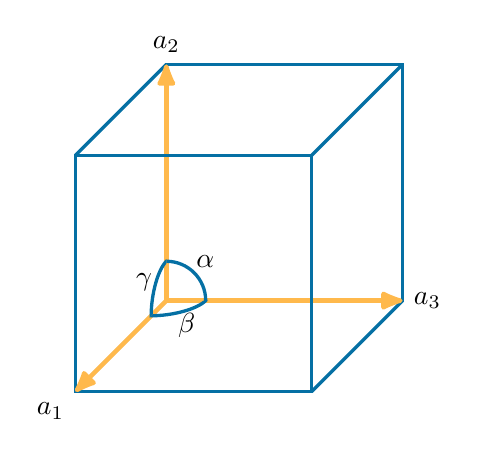
\begin{tikzpicture}
            \tikzset{edge/.style={highlight, very thick}}
            \tikzset{vector/.style={>={Latex[round]},
                    complementary, ultra thick, text=black}}
            \tikzset{angle/.style={highlight, very thick}}
            % Edges
            \draw[edge] (0, 0, 0) rectangle (3, 3, 0);
            \draw[edge] (0, 0, 3) rectangle (3, 3, 3);
            \draw[edge] (0, 0, 0) -- (0, 0, 3);
            \draw[edge] (0, 3, 0) -- (0, 3, 3);
            \draw[edge] (3, 0, 0) -- (3, 0, 3);
            \draw[edge] (3, 3, 0) -- (3, 3, 3);
            % Lattice vectors
            \draw[->, vector] (0, 0, 0) -- (0, 0, 3) node[below left] {\(\vv{a_1}\)};
            \draw[->, vector] (0, 0, 0) -- (0, 3, 0) node[above] {\(\vv{a_2}\)};
            \draw[->, vector] (0, 0, 0) -- (3, 0, 0) node[right] {\(\vv{a_3}\)};
            % Draw over lattice vectors where they cross under edges
            \draw[edge] (0, 3, 3) -- (3, 3, 3);
            \draw[edge] (3, 0, 3) -- (3, 3, 3);
            % Angles
            \begin{scope}[canvas is xy plane at z=0]
                \clip (0, 0) rectangle (1, 1);
                \draw[angle] circle [radius = 0.5];
                \node at (45:0.7) {\(\alpha\)};
            \end{scope}
            \begin{scope}[canvas is yz plane at x=0]
                \clip (0, 0) rectangle (1, 1);
                \draw[angle] circle [radius = 0.5];
                \node at (55:0.9) {\(\gamma\)};
            \end{scope}
            \begin{scope}[canvas is zx plane at y=0]
                \clip (0, 0) rectangle (1.2, 1.2);
                \draw[angle] circle [radius = 0.5];
                \node at (35:1) {\(\beta\)};
            \end{scope}
        \end{tikzpicture}
        \caption{A unit cell spanned by the lattice vectors \(\vv{a_1}\), \(\vv{a_2}\), and \(\vv{a_3}\).}
        \label{fig:unit cell}
    \end{figure}
    
    The volume of the unit cell is given by the scalar triple product:
    \begin{equation}
        V = \abs{\vv{a_1}\cdot (\vv{a_2}\times\vv{a_3})}
    \end{equation}

    \subsection{Symmetries}
    We can learn a lot about a crystal from the symmetries that it possess, or fails to posses.
    We can see the symmetry of many crystals from the shapes that they form.
    For example, cubic pyrite, \ce{FeS2}, forms cubic crystals.
    These have four-fold rotational symmetry about their faces, and also three fold rotational symmetry about their points.
    There are a few types of symmetry that are interesting for crystals and we shall discus these in this section.
    
    \subsubsection{Mirror Plane Symmetry}
    A \defineindex{mirror plane symmetry} means that there is a plane (or in two dimensions a line) through which we can reflect the object and the result is identical to having done nothing.
    For example a simple square has four mirror symmetries:
    \begin{equation*}
        \tikzsetnextfilename{mirror-symmetry-square}
        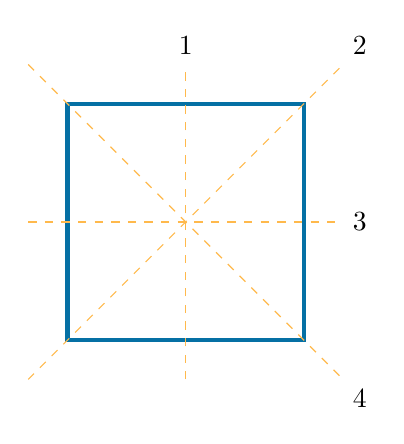
\begin{tikzpicture}
            \draw[highlight, ultra thick] (-1.5, -1.5) rectangle (1.5, 1.5);
            \draw[complementary, dashed, text=black] (0, -2) -- (0, 2) node[above] {1};
            \draw[complementary, dashed, text=black] (-2, 0) -- (2, 0) node[right] {3};
            \draw[complementary, dashed, text=black] (-2, -2) -- (2, 2) node[above right] {2};
            \draw[complementary, dashed, text=black] (-2, 2) -- (2, -2) node[below right] {4};
        \end{tikzpicture}
    \end{equation*}
    If we introduce another feature, such as dots, we reduce the number of symmetries:
    \begin{equation*}
        \tikzsetnextfilename{mirror-symmetry-dot-square}
        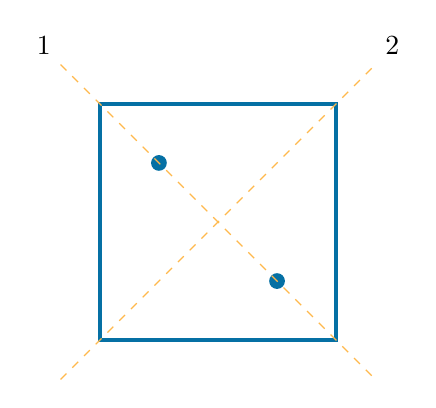
\begin{tikzpicture}
            \draw[highlight, ultra thick] (-1.5, -1.5) rectangle (1.5, 1.5);
            \fill[highlight] (-0.75, 0.75) circle [radius = 0.1];
            \fill[highlight] (0.75, -0.75) circle [radius = 0.1];
            \draw[complementary, dashed, text=black] (-2, -2) -- (2, 2) node[above right] {2};
            \draw[complementary, dashed, text=black] (-2, 2) -- (2, -2) node[above left, pos=0] {1};
        \end{tikzpicture}
    \end{equation*}
    
    A cube similarly has mirror plane symmetries, in fact, it has 9 of them. 
    This is shown in \cref{fig:mirror plane symmetry of a cube}.
    \begin{figure}
        \tikzsetnextfilename{mirror-plane-symmetry-cube}
        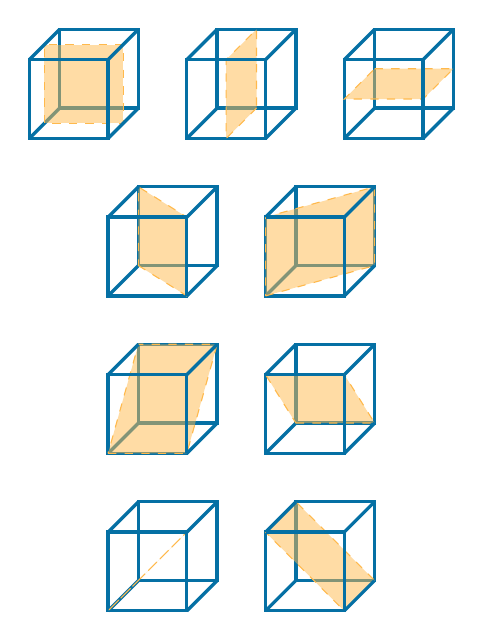
\begin{tikzpicture}
            \tikzset{edge/.style={highlight, very thick}}
            \tikzset{plane/.style={dashed, complementary, fill=complementary, fill opacity=0.5}}
            \draw[edge] (0, 0, 0) rectangle (1, 1, 0);
            \draw[edge] (0, 0, 1) rectangle (1, 1, 1);
            \draw[edge] (0, 0, 0) -- (0, 0, 1);
            \draw[canvas is xy plane at z=0.5, plane] (0, 0) rectangle (1, 1);
            \draw[edge] (0, 1, 0) -- (0, 1, 1);
            \draw[edge] (1, 0, 0) -- (1, 0, 1);
            \draw[edge] (1, 1, 0) -- (1, 1, 1);
            \draw[edge] (0, 1, 1) -- (1, 1, 1);
            \draw[edge] (1, 0, 1) -- (1, 1, 1);
            \begin{scope}[xshift=2cm]
                \draw[edge] (0, 0, 0) rectangle (1, 1, 0);
                \draw[edge] (0, 0, 1) rectangle (1, 1, 1);
                \draw[edge] (0, 0, 0) -- (0, 0, 1);
                \draw[canvas is yz plane at x=0.5, plane] (0, 0) rectangle (1, 1);
                \draw[edge] (0, 1, 0) -- (0, 1, 1);
                \draw[edge] (1, 0, 0) -- (1, 0, 1);
                \draw[edge] (1, 1, 0) -- (1, 1, 1);
                \draw[edge] (0, 1, 1) -- (1, 1, 1);
                \draw[edge] (1, 0, 1) -- (1, 1, 1);
            \end{scope}
            \begin{scope}[xshift=4cm]
                \draw[edge] (0, 0, 0) rectangle (1, 1, 0);
                \draw[edge] (0, 0, 1) rectangle (1, 1, 1);
                \draw[edge] (0, 0, 0) -- (0, 0, 1);
                \draw[canvas is zx plane at y=0.5, plane] (0, 0) rectangle (1, 1);
                \draw[edge] (0, 1, 0) -- (0, 1, 1);
                \draw[edge] (1, 0, 0) -- (1, 0, 1);
                \draw[edge] (1, 1, 0) -- (1, 1, 1);
                \draw[edge] (0, 1, 1) -- (1, 1, 1);
                \draw[edge] (1, 0, 1) -- (1, 1, 1);
            \end{scope}
            \begin{scope}[yshift=-2cm, xshift=1cm]
                \draw[edge] (0, 0, 0) rectangle (1, 1, 0);
                \draw[edge] (0, 0, 1) rectangle (1, 1, 1);
                \draw[edge] (0, 0, 0) -- (0, 0, 1);
                \draw[plane] (0, 0, 0) -- (1, 0, 1) -- (1, 1, 1) -- (0, 1, 0) -- cycle;
                \draw[edge] (0, 1, 0) -- (0, 1, 1);
                \draw[edge] (1, 0, 0) -- (1, 0, 1);
                \draw[edge] (1, 1, 0) -- (1, 1, 1);
                \draw[edge] (0, 1, 1) -- (1, 1, 1);
                \draw[edge] (1, 0, 1) -- (1, 1, 1);
            \end{scope}
            \begin{scope}[yshift=-2cm, xshift=3cm]
                \draw[edge] (0, 0, 0) rectangle (1, 1, 0);
                \draw[edge] (0, 0, 1) rectangle (1, 1, 1);
                \draw[edge] (0, 0, 0) -- (0, 0, 1);
                \draw[plane] (0, 0, 1) -- (1, 0, 0) -- (1, 1, 0) -- (0, 1, 1) -- cycle;
                \draw[edge] (0, 1, 0) -- (0, 1, 1);
                \draw[edge] (1, 0, 0) -- (1, 0, 1);
                \draw[edge] (1, 1, 0) -- (1, 1, 1);
                \draw[edge] (0, 1, 1) -- (1, 1, 1);
                \draw[edge] (1, 0, 1) -- (1, 1, 1);
            \end{scope}
            \begin{scope}[yshift=-4cm, xshift=1cm]
                \draw[edge] (0, 0, 0) rectangle (1, 1, 0);
                \draw[edge] (0, 0, 1) rectangle (1, 1, 1);
                \draw[edge] (0, 0, 0) -- (0, 0, 1);
                \draw[plane] (0, 0, 1) -- (1, 0, 1) -- (1, 1, 0) -- (0, 1, 0) -- cycle;
                \draw[edge] (0, 1, 0) -- (0, 1, 1);
                \draw[edge] (1, 0, 0) -- (1, 0, 1);
                \draw[edge] (1, 1, 0) -- (1, 1, 1);
                \draw[edge] (0, 1, 1) -- (1, 1, 1);
                \draw[edge] (1, 0, 1) -- (1, 1, 1);
            \end{scope}
            \begin{scope}[yshift=-4cm, xshift=3cm]
                \draw[edge] (0, 0, 0) rectangle (1, 1, 0);
                \draw[edge] (0, 0, 1) rectangle (1, 1, 1);
                \draw[edge] (0, 0, 0) -- (0, 0, 1);
                \draw[plane] (0, 0, 0) -- (1, 0, 0) -- (1, 1, 1) -- (0, 1, 1) -- cycle;
                \draw[edge] (0, 1, 0) -- (0, 1, 1);
                \draw[edge] (1, 0, 0) -- (1, 0, 1);
                \draw[edge] (1, 1, 0) -- (1, 1, 1);
                \draw[edge] (0, 1, 1) -- (1, 1, 1);
                \draw[edge] (1, 0, 1) -- (1, 1, 1);
            \end{scope}
            \begin{scope}[yshift=-6cm, xshift=1cm]
                \draw[edge] (0, 0, 0) rectangle (1, 1, 0);
                \draw[edge] (0, 0, 1) rectangle (1, 1, 1);
                \draw[edge] (0, 0, 0) -- (0, 0, 1);
                \draw[plane] (0, 0, 0) -- (0, 0, 1) -- (1, 1, 1) -- (1, 1, 0) -- cycle;
                \draw[edge] (0, 1, 0) -- (0, 1, 1);
                \draw[edge] (1, 0, 0) -- (1, 0, 1);
                \draw[edge] (1, 1, 0) -- (1, 1, 1);
                \draw[edge] (0, 1, 1) -- (1, 1, 1);
                \draw[edge] (1, 0, 1) -- (1, 1, 1);
            \end{scope}
            \begin{scope}[yshift=-6cm, xshift=3cm]
                \draw[edge] (0, 0, 0) rectangle (1, 1, 0);
                \draw[edge] (0, 0, 1) rectangle (1, 1, 1);
                \draw[edge] (0, 0, 0) -- (0, 0, 1);
                \draw[plane] (1, 0, 0) -- (1, 0, 1) -- (0, 1, 1) -- (0, 1, 0) -- cycle;
                \draw[edge] (0, 1, 0) -- (0, 1, 1);
                \draw[edge] (1, 0, 0) -- (1, 0, 1);
                \draw[edge] (1, 1, 0) -- (1, 1, 1);
                \draw[edge] (0, 1, 1) -- (1, 1, 1);
                \draw[edge] (1, 0, 1) -- (1, 1, 1);
            \end{scope}
        \end{tikzpicture}
        \caption{Mirror plane symmetries of a cube, there are 9 in total.}
        \label{fig:mirror plane symmetry of a cube}
    \end{figure}
    
    \subsubsection{Rotational Symmetry}
    An object has \(k\)-fold \defineindex{rotational symmetry} about some axis, \(\vh{n}\) if it is possible to rotate the object by some multiple of \(2\pi/k\) about \(\vh{n}\) and it looks like nothing has happened.
    For example, \cref{fig:rotational symmetry star} shows a five pointed star with 5-fold rotational symmetry, including a rotation by 0 or \(2\pi\), which is equivalent to doing nothing.\footnote{The symmetry group is \(\integers_5\), or more generally for a \(k\)-fold rotationally symmetric object, \(\integers_k\).}
    
    \begin{figure}
        \tikzsetnextfilename{rotational-symmetry-star}
        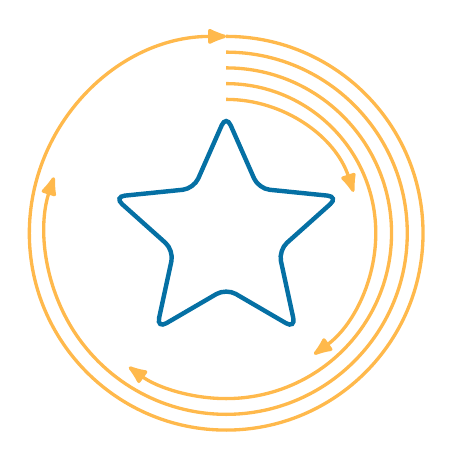
\begin{tikzpicture}
            \node[star, draw, minimum size=3cm, ultra thick, highlight, star point height=0.8cm, rounded corners] {};
            \draw[-{Latex[round]}, very thick, complementary] (90:1.7) arc (90:18:1.7);
            \draw[-{Latex[round]}, very thick, complementary] (90:1.9) arc (90:-54:1.9);
            \draw[-{Latex[round]}, very thick, complementary] (90:2.1) arc (90:-126:2.1);
            \draw[-{Latex[round]}, very thick, complementary] (90:2.3) arc (90:-198:2.3);
            \draw[-{Latex[round]}, very thick, complementary] (90:2.5) arc (90:-270:2.5);
        \end{tikzpicture}
        \caption{A five pointed star has 5-fold rotational symmetry, including a rotation by \(0\) or \(2\pi\), which is the identity, in that it leaves the shape completely the same.}
        \label{fig:rotational symmetry star}
    \end{figure}

    A square has four-fold rotational symmetry.\footnote{The dihedral group, \(D_4\), is the symmetry group of a square combining the rotational and reflective symmetries.}
    A cube also has rotational symmetries, but in three dimensions things are more complicated as we have far more choices of axes of rotation.
    \Cref{fig:rotational symmetry cube} shows a cube with three axes of rotational symmetry.
    The first connects two diagonally opposite corners.
    The cube has three-fold rotational symmetry about this axis.
    The second connects the mid points of two diagonally opposite edges.
    The cube has two-fold rotational symmetry about this axis.
    The third connects the centre of two opposite faces.
    The cube has four-fold rotational symmetry about this axis.
    There are four axes of the first type, six of the second type, and three of the third type, for 13 total axes of rotation.
    
    \begin{figure}
        \tikzsetnextfilename{rotational-symmetry-cube}
        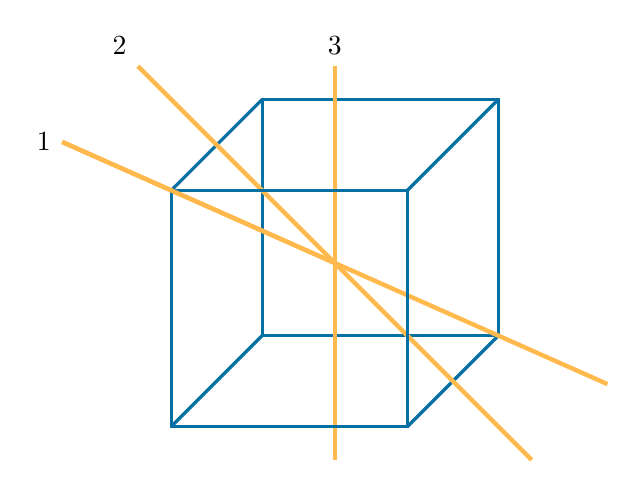
\begin{tikzpicture}
            \tikzset{edge/.style={very thick, highlight}}
            \draw[edge] (0, 0, 0) rectangle (3, 3, 0);
            \draw[edge] (0, 0, 0) -- (0, 0, 3);
            \draw[edge] (3, 3, 0) -- (3, 3, 3);
            \draw[edge] (0, 3, 0) -- (0, 3, 3);
            \draw[edge] (3, 0, 0) -- (3, 0, 3);
            \draw[edge] (2.5, 0, 0) -- (3, 0, 0) -- (3, 0.5, 0);
            \draw[ultra thick, complementary, text=black] (1.5, -1, 1.5) -- (1.5, 4, 1.5) node[above] {3};
            \draw[ultra thick, complementary, text=black] (-1, 4, 4) -- (4, -1, -1) node[left, pos=0] {1};
            \draw[ultra thick, complementary, text=black] (-1, 4, 1.5) -- (4, -1, 1.5) node[above left, pos=0] {2};
            \draw[edge] (0, 0, 3) rectangle (3, 3, 3);
            \draw[ultra thick, complementary, text=black] (-1, 4, 4) -- (1.5, 1.5, 1.5);
        \end{tikzpicture}
        \caption{Three possible axes of rotational symmetry of the cube.}
        \label{fig:rotational symmetry cube}
    \end{figure}
    
    \subsubsection{Inversion}
    An \defineindex{inversion symmetry} is reflection through a point, called the \defineindex{centre of inversion}, which leaves the object unchanged.
    For example, this graph,
    \begin{equation*}
        \tikzsetnextfilename{inversion-symmetry-plane}
        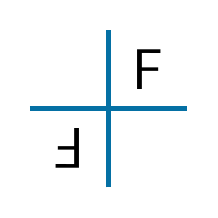
\begin{tikzpicture}
            \draw[highlight, ultra thick] (-1, 0) -- (1, 0);
            \draw[highlight, ultra thick] (0, -1) -- (0, 1);
            \node at (0.5, 0.5) {\huge\textsf{\textsf{F}}};
            \node[rotate around={180:(0,0)}] at (-0.5, -0.5) {\huge\textsf{\textsf{F}}};
        \end{tikzpicture}
    \end{equation*}
    has a centre of inversion at the origin.
    
    This tetrahedron,
    \begin{equation*}
        \tikzsetnextfilename{inversion-symmetry-tetrahedron}
        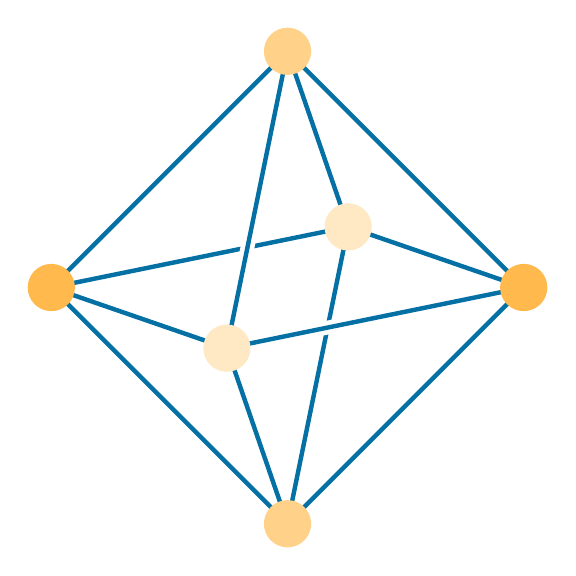
\begin{tikzpicture}
            \tikzset{edge/.style={ultra thick, highlight}}
            \tikzset{under edge/.style={line width=5pt, white}}
            \draw[edge] (3, 0, -2) -- (3, -3, 0);
            \draw[under edge] (3, 0, 2) -- (6, 0, 0);
            \draw[edge] (0, 0, 0) -- (3, 0, 2) -- (6, 0, 0) -- (3, 0, -2) -- cycle;
            \draw[edge] (0, 0, 0) -- (3, 3, 0);
            \draw[under edge] (3, 0, 2) -- (3, 3, 0);
            \draw[edge] (3, 0, 2) -- (3, 3, 0);
            \draw[edge] (6, 0, 0) -- (3, 3, 0);
            \draw[edge] (3, 0, -2) -- (3, 3, 0);
            \draw[edge] (0, 0, 0) -- (3, -3, 0);
            \draw[edge] (3, 0, 2) -- (3, -3, 0);
            \draw[edge] (6, 0, 0) -- (3, -3, 0);
            
            \fill[complementary] (0, 0, 0) circle [radius = 0.3];
            \fill[complementary] (6, 0, 0) circle [radius = 0.3];
            \fill[complementary!33] (3, 0, 2) circle [radius = 0.3];
            \fill[complementary!33] (3, 0, -2) circle [radius = 0.3];
            \fill[complementary!66] (3, 3, 0) circle [radius = 0.3];
            \fill[complementary!66] (3, -3, 0) circle [radius = 0.3];
        \end{tikzpicture}
    \end{equation*}
    has a centre of inversion at its centre.
    The corresponding symmetry swaps points of the same shade.
    
    A cube has a centre of inversion at its centre.
    Combining this with the 9 mirror plane symmetries and 13 rotational symmetries we see a cube has 24 symmetries to consider.
    
    \subsection{Symmetry Applications to Crystals}
    Suppose a crystal has four-fold rotational symmetry.
    It is not difficult to convince yourself that this can only be the case if \(\abs{\vv{a_1}} = \abs{\vv{a_2}}\) and \(\angle(\vv{a_1}, \vv{a_2}) = \pi/2\).
    We call this a square lattice for obvious reasons.
    
    If we only require two-fold rotational symmetry then we can relax the condition on the vector lengths and we get a rectangular lattice, which has \(\abs{\vv{a_1}} \ne \abs{\vv{a_2}}\) and \(\angle(\vv{a_1},\vv{a_2}) = \pi/2\).
    
    The symmetry imposes conditions on the lattice parameters.
    Similarly if a crystal has three-fold rotational symmetry then this necessitates that \(\abs{\vv{a_1}} = \abs{\vv{a_2}}\) and \(\angle(\vv{a_1}, \vv{a_2}) = 2\pi/3\).
    We call this a hexagonal lattice as three unit cells together form a regular hexagon.
    
    These three lattices, along with relevant unit cells, are shown in \cref{fig:square rectangle hexagon lattice}, as well as the three unit cells forming a hexagon in the hexagonal lattice.
    
    \begin{figure}
        \tikzsetnextfilename{square-rectangle-hexagon-lattice}
        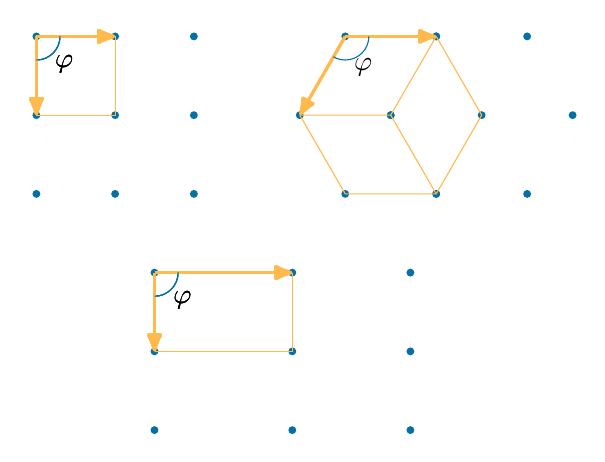
\begin{tikzpicture}
            \foreach \x in {0,..., 2} {
                \foreach \y in {0,..., 2} {
                    \fill[highlight] (\x, \y) circle [radius = 0.05];
                }
                \draw[very thick, complementary, -{Latex[round]}] (0, 2) -- (1, 2);
                \draw[very thick, complementary, -{Latex[round]}] (0, 2) -- (0, 1);
                \draw[complementary] (0, 1) -- (1, 1) -- (1, 2);
                \begin{scope}
                    \clip (0, 2) rectangle (1, 1);
                    \draw[highlight] (0, 2) circle [radius = 0.3];
                \end{scope}
                \node at ($(0, 2) + (-45:0.5)$) {\(\varphi\)};
            }
            \begin{scope}[xshift=3.5cm]
                \fill[highlight] (1, 1) circle [radius = 0.05];
                \foreach \a in {0, 60,..., 300} {
                    \fill[highlight] ($(1, 1) + (\a:1.155)$) circle [radius = 0.05];
                    \fill[highlight] ($(1, 1) + (\a:1.155) + (0:1.155)$) circle [radius = 0.05];
                }
                \draw[very thick, complementary, -{Latex[round]}] ($(1, 1) + (120:1.155)$) -- ($(1, 1) + (60:1.155)$);
                \draw[very thick, complementary, -{Latex[round]}] ($(1, 1) + (120:1.155)$) -- ($(1, 1) + (180:1.155)$);
                \draw[complementary] ($(1, 1) + (180:1.155)$) -- ($(1, 1) + (240:1.155)$) -- ($(1, 1) + (300:1.155)$) -- ($(1, 1) + (0:1.155)$) -- ($(1, 1) + (60:1.155)$);
                \draw [complementary] ($(1, 1) + (180:1.155)$) -- (1, 1) -- ($(1, 1) + (-60:1.155)$);
                \draw [complementary] (1, 1) -- ($(1, 1) + (60:1.155)$);
                \begin{scope}
                    \clip ($(1, 1) + (120:1.155)$) -- ($(1, 1) + (60:1.155)$) -- (1, 1) -- ($(1, 1) + (180:1.155)$) -- cycle;
                    \draw[highlight] ($(1, 1) + (120:1.155)$) circle [radius = 0.3];
                    \node at ($(1, 1) + (120:0.70)$) {\(\varphi\)};
                \end{scope}
            \end{scope}
            \begin{scope}[xshift=1.5cm, yshift=-3cm]
                \foreach \x in {0, 1.75, 3.25} {
                    \foreach \y in {0,..., 2} {
                        \fill[highlight] (\x, \y) circle [radius = 0.05];
                    }
                    \draw[very thick, complementary, -{Latex[round]}] (0, 2) -- (1.75, 2);
                    \draw[very thick, complementary, -{Latex[round]}] (0, 2) -- (0, 1);
                    \draw[complementary] (0, 1) -- (1.75, 1) -- (1.75, 2);
                    \begin{scope}
                        \clip (0, 2) rectangle (1.75, 1);
                        \draw[highlight] (0, 2) circle [radius = 0.3];
                    \end{scope}
                    \node at ($(0, 2) + (-45:0.5)$) {\(\varphi\)};
                }
            \end{scope}
        \end{tikzpicture}
        \caption{A square lattice (top left), hexagonal lattice (top right), and hexagonal lattice (bottom). For the square and rectangular lattices \(\varphi = \pi/2\) and for the hexagonal lattice \(\varphi = 2\pi/3\). For the square and hexagonal lattice \(\abs{\vv{a_1}} = \abs{\vv{a_2}}\).}
        \label{fig:square rectangle hexagon lattice}
    \end{figure}
    
    What we are discussing are two-dimensional lattices.
    The three we have discussed are the result of symmetry restrictions.
    There is also a lattice that results from no symmetry restrictions, called the centred rectangular lattice.
    This is shown in \cref{fig:centred rectangular lattice}.
    The primitive unit cell shown is awkward to work with and doesn't lead to much insight.
    If we allow ourselves to work with non-primitive unit cells then the second unit cell shown is a more sensible choice.
    This is called a centred rectangular unit cell, since it is rectangular and has a lattice point at its centre.
    
    \begin{figure}
        \tikzsetnextfilename{centred-rectangular-lattice}
        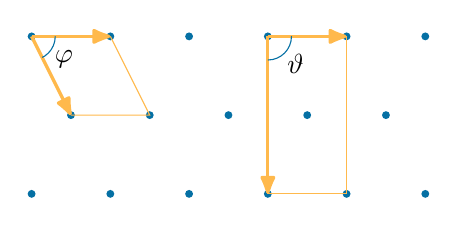
\begin{tikzpicture}
            \foreach \x in {0,...,4} {
                \fill[highlight] (\x + 1, 0) circle [radius = 0.05];
                \fill[highlight] (\x + 0.5, 1) circle [radius = 0.05];
                \fill[highlight] (\x, 2) circle [radius = 0.05];
            }
            \fill[highlight] (0, 0) circle [radius = 0.05];
            \fill[highlight] (5, 2) circle [radius = 0.05];
            \draw[very thick, complementary, -{Latex[round]}] (0, 2) -- (1, 2);
            \draw[very thick, complementary, -{Latex[round]}] (0, 2) -- (0.5, 1);
            \draw[complementary] (0.5, 1) -- (1.5, 1) -- (1, 2);
            \begin{scope}
                \clip (0, 2) -- (1, 2) -- (1.5, 1) -- (0.5, 1) -- cycle;
                \draw[highlight] (0, 2) circle [radius = 0.3];
            \end{scope}
            \node at ($(0, 2) + (-35:0.5)$) {\(\varphi\)};
            \draw[very thick, complementary, -{Latex[round]}] (3, 2) -- (3, 0);
            \draw[very thick, complementary, -{Latex[round]}] (3, 2) -- (4, 2);
            \draw[complementary] (3, 2) rectangle (4, 0);
            \begin{scope}
                \clip (3, 2) rectangle (4, 0);
                \draw[highlight] (3, 2) circle [radius = 0.3];
            \end{scope}
            \node at ($(3, 2) + (-45:0.5)$) {\(\vartheta\)};
        \end{tikzpicture}
        \caption{The centred rectangular lattice with its primitive unit cell and the simpler choice of a centred rectangular unit cell.}
        \label{fig:centred rectangular lattice}
    \end{figure}
    
    The four two-dimensional lattices we have seen cover all possible cases.
    These are together known as the two-dimensional \defineindex{Bravais lattices}.
    They are summarised in \cref{tab:2d bravais lattices}.
    
    \begin{table}
        \caption{The key information about two-dimensional Bravais lattices.}
        \label{tab:2d bravais lattices}
        \begin{tabular}{lll}
            \toprule
            Crystal & External Minimum Symmetry & Restrictions\\ \midrule
            \multirow{2}{*}{Square} & \multirow{2}{*}{Four-fold rotational symmetry} & \(\abs{\vv{a_1}} = \abs{\vv{a_2}}\)\\
            && \(\angle(\vv{a_1},\vv{a_2}) = \pi/2\)\\\midrule
            Rectangular & Two-fold rotational symmetry & \(\angle(\vv{a_1},\vv{a_2}) = \pi/2\)\\\midrule
            \multirow{2}{*}{Hexagonal} & \multirow{2}{*}{Three-fold rotational symmetry} & \(\abs{\vv{a_1}} = \abs{\vv{a_2}}\)\\
            && \(\angle(\vv{a_1},\vv{a_2}) = 2\pi/3\)\\
            Centred Rectangular & None & None\\
            \bottomrule
        \end{tabular}
    \end{table}
    
    In three dimensions we can make similar arguments about symmetries and the resulting restrictions on the lattice parameters.
    We end up with a list of seven three-dimensional Bravais lattices.
    The key information for these is in \cref{tab:3d bravais lattices}.
    
    \begin{table}
        \caption{The key information about three-dimensional Bravais lattices.}
        \label{tab:3d bravais lattices}
        \begin{tabular}{lll}\toprule
            Crystal & External Minimum Symmetry & Restrictions\\\midrule
            \multirow{2}{*}{Cubic} & \multirow{2}{*}{\parbox{4.4cm}{Four three-fold rotational symmetries}} & \(a = b = c\)\\
            && \(\alpha = \beta = \gamma = \pi/2\)\\\midrule
            \multirow{2}{*}{Hexagonal} & \multirow{2}{*}{\parbox{4.4cm}{One six-fold rotational symmetry}} & \(a = b\), \(\gamma = 2\pi/3\)\\
            && \(\alpha = \beta = \pi/2\)\\\midrule
            \multirow{3}{*}{Trigonal} & \multirow{3}{*}{\parbox{4.4cm}{One three-fold rotational symmetry}} & \(a = b = c\)\\
            && \(\alpha = \beta = \gamma \le 2\pi/3\)\\
            && \(\alpha \ne \pi/2\)\\\midrule
            \multirow{2}{*}{Tetragonal} & \multirow{2}{*}{\parbox{4.4cm}{One four-fold rotational symmetry}} & \(a = b\)\\
            && \(\alpha = \beta = \gamma = \pi/2\)\\\midrule
            Orthorhombic & \parbox{4.4cm}{Three perpendicular two-fold rotational symmetries} & \(\alpha = \beta = \gamma = \pi/2\)\\\midrule
            Monoclinic & \parbox{4.4cm}{One two-fold rotational symmetry, parallel to \(b\)} & \(\alpha = \gamma = \pi/2 \ne \beta\)\\\midrule
            Triclinic & None & None\\\bottomrule
        \end{tabular}
    \end{table}
    
    This isn't quite the complete picture however as we have assumed these are all primitive unit cells.
    In three dimensions there are actually four centrings, where we add additional lattice points to the unit cell, to consider.
    The first, and simplest, is the primitive unit cell, P.
    The second is face centring, F, where we add an extra lattice point to every face.
    The third is body centring, I, where we add an extra lattice point to the centre of the cell (I for interior).
    The fourth is base centred, denoted either A, B, or C, where we add an extra lattice point to one pair of opposite faces.
    If we add to the face spanned by \(\vv{a_1}\) and \(\vv{a_2}\) then we call it C, the face spanned by \(\vv{a_1}\) and \(\vv{a_3}\) corresponds to B, and the face spanned by \(\vv{a_2}\) and \(\vv{a_3}\) corresponds to A.
    Not all crystal system and centring pairings give us a useful lattice however.
    The ones that do are given in \cref{tab:crystal system centring}.
    We are now in a position to fully specify a crystal lattice by stating the crystal structure and the centring.
    \begin{table}
        \caption{Crystal systems and centrings. Note that R stands for rhombohedral, a trigonal crystal can be categorised as having either a hexagonal or rhombohedral lattice system}
        \label{tab:crystal system centring}
        \begin{tabular}{ll}\toprule
            Crystal System & Centring\\\midrule
            Cubic & P, F, and I\\
            Hexagonal & P\\
            Trigonal & P, and R\\
            Tetragonal & P, and I\\
            Orthorhombic & P, I, and F\\
            Monoclinic & P, and A/B/C\\
            Triclinic & P\\\bottomrule
        \end{tabular}
    \end{table}

    \subsection{Basis}
    Now that we can fully specify a crystal lattice we need to use this to define a crystal.
    We do this with the help of a basis, which is a list of atoms and locations that they occur in the unit cell.
    We typically give these locations in dimensionless, reduced coordinates, \((x, y, z)\), corresponding to the position
    \begin{equation}
        \vv{r} = x\vv{a_1} + y\vv{a_2} + z\vv{a_3}
    \end{equation}
    The simplest basis is to have only a single atom at \(\vv{r} = (0, 0, 0)\).
    This is the case with many pure metals, for example \ce{Na}, \ce{Ba}, and \ce{Fe} all have body-centred cubic lattices (BCC)\glossary[acronym]{BCC}{body-centred cubic} with this basis, and \ce{Ca}, \ce{Ni}, and \ce{Au} have face-centred cubic lattices (FCC)\glossary[acronym]{FCC}{face-centred cubic} with this basis.
    It is worth looking at these examples in more detail.
    
    \subsubsection{Body-Centred Cubic}
    A body-centred cubic lattice unit cell consists of lattice points at the eight corners of a cube, and one lattice point in the middle.
    We consider the case of the basis being a single atom at \((0, 0, 0)\).
    The conventional lattice vectors in this case are \(\vv{a_1} = a\vh{x}\), \(\vv{a_2} = a\vh{y}\), and \(\vv{a_3} = a\vh{z}\), where \(\vh{x}\), \(\vh{y}\), and \(\vh{z}\) are orthonormal Cartesian unit vectors.
    There are two atoms in the conventional unit cell, one at the centre, and 1/8 of an atom in each corner, these are shared between the neighbouring cells.
    The positions of the atoms in reduced coordinates in the unit cell are \((0, 0, 0)\) and \((1/2, 1/2, 1/2)\).
    Each atom has 8 nearest neighbours and 6 next-nearest neighbours.
    
    The primitive unit cell is more complicated so we don't use it often but it has lattice vectors
    \begin{equation}
        \vv{a_1^P} = \frac{a}{2}(-\vh{x} + \vh{y} + \vh{z}), \qquad \vv{a_2^P} = \frac{a}{2}(\vh{x} - \vh{y} + \vh{z}), \qqand \vv{a_3^P} = \frac{a}{2}(\vh{x} + \vh{y} - \vh{z}).
    \end{equation}
    It is clear why one would prefer a centred cubic lattice over this oddly shaped primitive lattice.
    
    \begin{figure}
        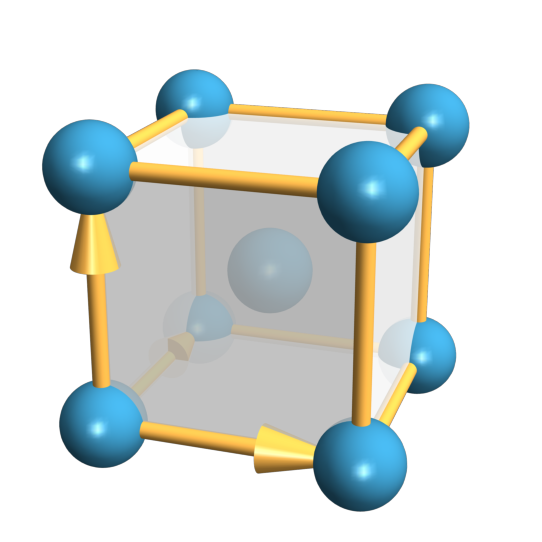
\includegraphics{images/bcc-crystal.pdf}
        \caption{A body-centred crystal.}
    \end{figure}
    
    \subsubsection{Face-Centred Cubic}
    A face-centred cubic lattice unit cell consists of a lattice point at the eight corners of a cube, and one lattice point in the centre of each face.
    We consider the case of a basis of a single atom at \((0, 0, 0)\).
    The conventional lattice vectors in this case are \(\vv{a_1} = a\vh{x}\), \(\vv{a_2} = a\vh{y}\), and \(\vv{a_3} = a\vh{z}\), where \(\vh{x}\), \(\vh{y}\), and \(\vh{z}\) are orthonormal Cartesian unit vectors.
    There are four atoms in the conventional unit cell.
    Each of the six faces contributes half an atom, and the four corners contribute 1/8 of an atom.
    The positions of the atoms in reduced coordinates are \((0, 0, 0)\) and \((1/2, 0, 0)\).
    Each atom has 12 nearest neighbours.
    
    The primitive unit cell is more complicated so we don't use it often but it has lattice vectors
    \begin{equation}
        \vv{a_1^P} = \frac{a}{2}(\vh{y} + \vh{z}), \qquad \vv{a_2^P} = \frac{a}{2}(\vh{x} + \vh{z}), \qqand \vv{a_3^P} = \frac{a}{2}(\vh{x} + \vh{y}).
    \end{equation}
    It is clear why one would prefer a centred cubic lattice over this oddly shaped primitive lattice.
    
    The face-centred cubic lattice is the densest possible way to pack of hard, non-overlapping spheres.
    For this reason it is also called \defineindex{cubic close packed} (CCP)\glossary[acronym]{CCP}{cubic close-packed}.
    
    \begin{figure}
        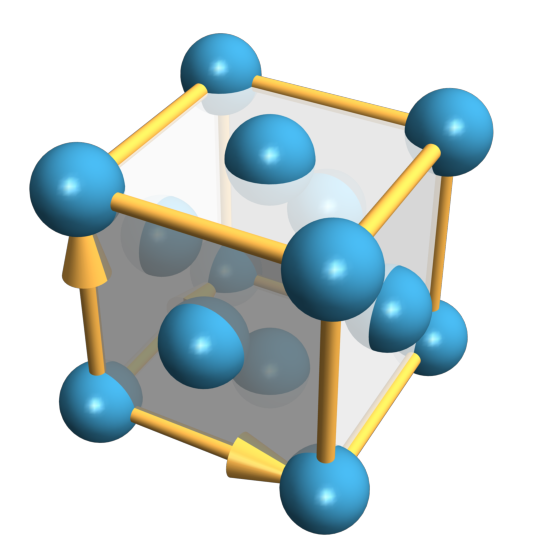
\includegraphics{images/fcc-crystal.pdf}
        \caption{A face-centred crystal.}
    \end{figure}
    
    \subsubsection{Hexagonal Close-Packed}
    A hexagonal close-packed (HCP)\glossary[acronym]{HCP}{hexagonal close-packed} consists of a hexagonal unit cell, with lattice parameters \(a = b\) and \(\gamma = 2\pi/3\).
    There are two atoms in the conventional unit cell, positioned at \((2/3,1/3,1/4)\) and \((1/3,2/3,3/4)\).
    Each atom has 12 nearest neighbours.
    The packing density of this structure is equal to that of cubic close-packing.
    There is no conventional choice of lattice vectors, but one option is
    \begin{equation}
        \vv{a_1} = a\frac{\sqrt{3}}{2}\vh{x} + \frac{a}{2}\vh{y}, \qquad \vv{a_2} = -a\frac{\sqrt{3}}{2}\vh{x} + \frac{a}{2}\vh{y}, \qqand \vv{a_3} = c\vh{z}.
    \end{equation}

    \subsubsection{Close Packing}
    Both cubic and hexagonal close packing can be created by layering hexagonally arranged layers of spheres.
    The difference comes in where you choose to place the third layer.
    If you choose to place the third layer such that it lines up with the first layer then the result will be hexagonal close packing.
    If you choose instead to place it so that it doesn't line up you will get cubic close-packing.
    
    \subsubsection{Real Life Example}
    Consider \ce{NaCl}, common table salt, this has a face-centred cubic lattice.
    We need to choose an atom type to have at the position \((0, 0, 0)\), we arbitrarily choose \ce{Cl}.
    The basis is then a \ce{Cl} atom at \((0, 0, 0)\) and a \ce{Na} atom at \((1/2,0,0)\), or equivalently at \((1/2,1/2,1/2)\).
    
    Crystals can become very complicated in the real world but they can always be broken down into a choice of lattice and centring and a basis of atoms.
    
    \chapter{Crystal Planes}
    \section{What Are They, and Why Do We Care?}
    Crystal planes are sets of parallel planes upon which all of the atoms in a crystal can be located.
    The nature of the planes in a crystal can be important for its physical properties.
    The most obvious example being diffraction, and in particular Bragg's law, which predicts from the spacing between parallel planes what diffraction pattern will occur.
    We will see this later when we consider diffraction in more detail.
    
    Transport properties (such as conductivity, both thermal and electrical) are also dependent on planes.
    Some materials have anisotropic transport properties, that is they may be better at transport in one direction.
    For example, graphite is made of layers of planes in which the atoms are arranged hexagonally.
    Graphite is a much better as an electrical and thermal conductor along the planes rather than across the planes.
    
    Planes can also be important for the for structural properties of materials.
    A crystal is much more likely to break along a plane and plastic deformation, such as a metal being permanently bent, most often occurs when planes slip past each other.
    
    The crystal planes also effect the surface properties of a crystal.
    For example, they may effect the ability of the crystal to act as a catalyst or semiconductor.
    
    \section{Describing Planes}
    \defineindex{Miller indices} provide a standard method of naming planes.
    The naming scheme goes as follows.
    First, find where the plane intersects each axis in reduced units, say, at \((3, 2, 2)\).
    If there is no intercept then we say the intercept occurs at \(\infty\), and we take \(1/\infty = 0\).
    Second, take the reciprocals, so for our example, \((1/3, 1/2, 1/2)\).
    Third, multiply through by the smallest integer that leaves all whole numbers, in our case this is six and we get \(\crystalplane{2}{3}{3}\).
    This is the name of our plane.
    If there is a negative number then we denote this with a bar above of the number.
    
    The crystal plane \(\crystalplane{h}{k}{\ell}\) intercepts the real space axes at \(\vv{a_1}/h\), \(\vv{a_2}/k\), and \(\vv{a_3}/\ell\).
    
    The Miller indices don't represent a single plane but an infinite family of parallel planes.
    
    We can also use Miller indices to denote a direction in a crystal.
    We denote by \(\crystaldirection{h}{k}{\ell}\) the direction \(h\vv{a_1} + k\vv{a_2} + \ell\vv{a_3}\).
    In cubic, tetragonal, and orthorhombic lattices, where all angles are \(\pi/2\), the direction \(\crystaldirection{h}{k}{\ell}\) is simply the direction perpendicular to the plane \(\crystalplane{h}{k}{\ell}\).
    
    \begin{figure}
        \tikzsetnextfilename{crystal-planes}
        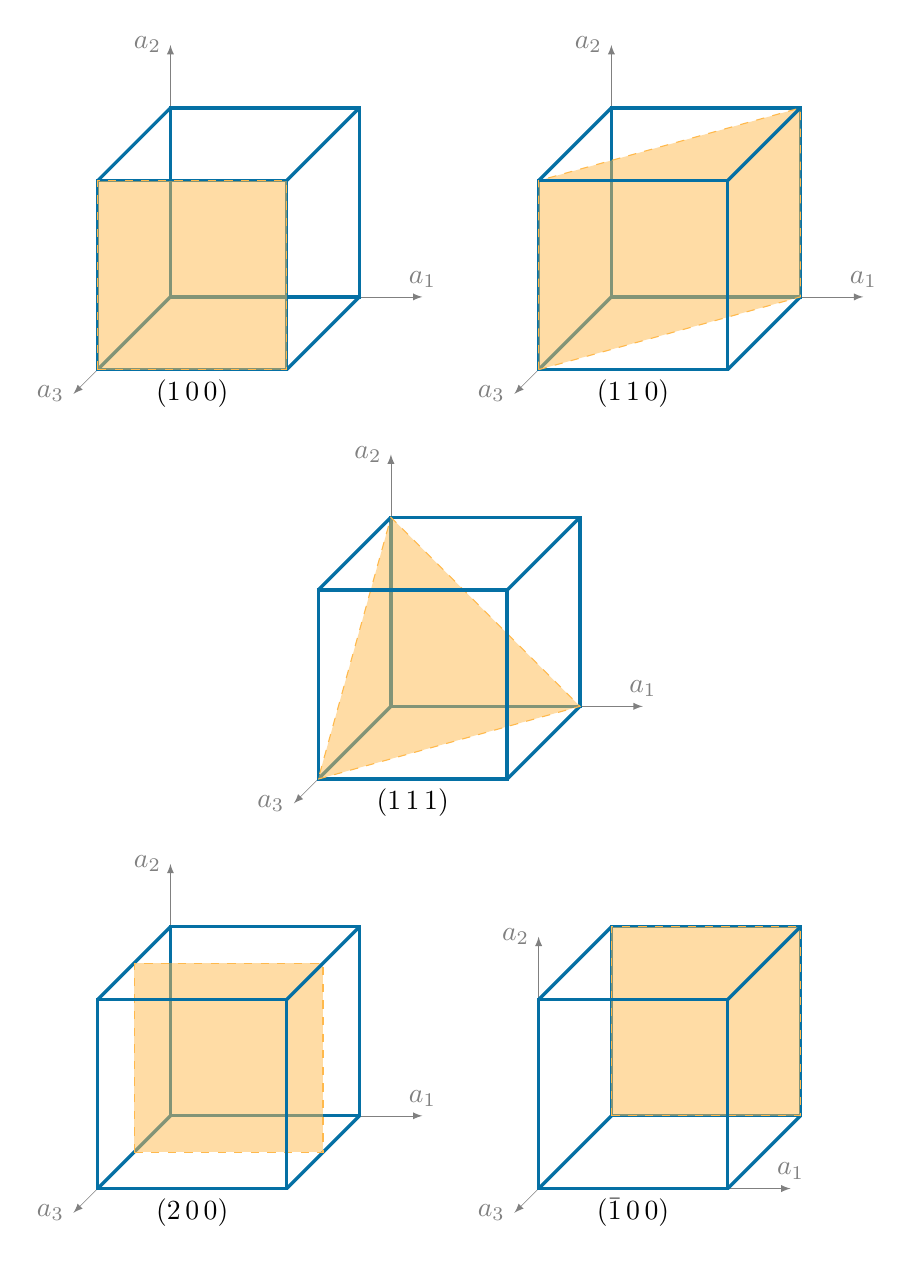
\begin{tikzpicture}[scale=0.8]
            \tikzset{edge/.style = {highlight, very thick}}
            \tikzset{plane/.style={dashed, complementary, fill=complementary, fill opacity=0.5}}
            \tikzset{axis/.style={help lines, ->}}
            \draw[axis] (0, 0, 0) -- (4, 0, 0) node[above] {\(\vv{a_1}\)};
            \draw[axis] (0, 0, 0) -- (0, 4, 0) node[left] {\(\vv{a_2}\)};
            \draw[axis] (0, 0, 0) -- (0, 0, 4) node[left] {\(\vv{a_3}\)};
            \draw[edge] (0, 0, 0) rectangle (3, 3, 0);
            \draw[edge] (0, 0, 3) rectangle (3, 3, 3);
            \draw[edge] (0, 0, 0) -- (0, 0, 3);
            \draw[edge] (0, 3, 0) -- (0, 3, 3);
            \draw[edge] (3, 0, 0) -- (3, 0, 3);
            \draw[edge] (3, 3, 0) -- (3, 3, 3);
            \draw[plane] (0, 0, 3) rectangle (3, 3, 3);
            \node[below] at (1.5, 0, 3) {\(\crystalplane{1}{0}{0}\)};
            \begin{scope}[xshift=7cm]
                \draw[axis] (0, 0, 0) -- (4, 0, 0) node[above] {\(\vv{a_1}\)};
                \draw[axis] (0, 0, 0) -- (0, 4, 0) node[left] {\(\vv{a_2}\)};
                \draw[axis] (0, 0, 0) -- (0, 0, 4) node[left] {\(\vv{a_3}\)};
                \draw[edge] (0, 0, 0) rectangle (3, 3, 0);
                \draw[edge] (0, 0, 3) rectangle (3, 3, 3);
                \draw[edge] (0, 0, 0) -- (0, 0, 3);
                \draw[edge] (0, 3, 0) -- (0, 3, 3);
                \draw[edge] (3, 0, 0) -- (3, 0, 3);
                \draw[plane] (0, 0, 3) -- (3, 0, 0) -- (3, 3, 0) -- (0, 3, 3) -- cycle;
                \draw[edge] (3, 3, 0) -- (3, 3, 3);
                \draw[edge] (0, 3, 3) -- (3, 3, 3);
                \draw[edge] (3, 0, 3) -- (3, 3, 3);
                \node[below] at (1.5, 0, 3) {\(\crystalplane{1}{1}{0}\)};
            \end{scope}
            \begin{scope}[xshift=3.5cm, yshift=-6.5cm]
                \draw[axis] (0, 0, 0) -- (4, 0, 0) node[above] {\(\vv{a_1}\)};
                \draw[axis] (0, 0, 0) -- (0, 4, 0) node[left] {\(\vv{a_2}\)};
                \draw[axis] (0, 0, 0) -- (0, 0, 4) node[left] {\(\vv{a_3}\)};
                \draw[edge] (0, 0, 0) rectangle (3, 3, 0);
                \draw[edge] (0, 0, 3) rectangle (3, 3, 3);
                \draw[edge] (0, 0, 0) -- (0, 0, 3);
                \draw[edge] (0, 3, 0) -- (0, 3, 3);
                \draw[edge] (3, 0, 0) -- (3, 0, 3);
                \draw[edge] (3, 3, 0) -- (3, 3, 3);
                \draw[plane] (0, 0, 3) -- (3, 0, 0) -- (0, 3, 0) -- cycle;
                \node[below] at (1.5, 0, 3) {\(\crystalplane{1}{1}{1}\)};
                \draw[edge] (0, 3, 3) -- (3, 3, 3);
                \draw[edge] (3, 0, 3) -- (3, 3, 3);
            \end{scope}
            \begin{scope}[yshift=-13cm]
                \draw[axis] (0, 0, 0) -- (4, 0, 0) node[above] {\(\vv{a_1}\)};
                \draw[axis] (0, 0, 0) -- (0, 4, 0) node[left] {\(\vv{a_2}\)};
                \draw[axis] (0, 0, 0) -- (0, 0, 4) node[left] {\(\vv{a_3}\)};
                \draw[edge] (0, 0, 0) rectangle (3, 3, 0);
                \draw[edge] (0, 0, 3) rectangle (3, 3, 3);
                \draw[edge] (0, 0, 0) -- (0, 0, 3);
                \draw[edge] (0, 3, 0) -- (0, 3, 3);
                \draw[edge] (3, 0, 0) -- (3, 0, 3);
                \draw[plane] (0, 0, 1.5) rectangle (3, 3, 1.5);
                \node[below] at (1.5, 0, 3) {\(\crystalplane{2}{0}{0}\)};
                \draw[edge] (0, 3, 3) -- (3, 3, 3);
                \draw[edge] (3, 0, 3) -- (3, 3, 3);
                \draw[edge] (3, 3, 0) -- (3, 3, 3);
            \end{scope}
            \begin{scope}[yshift=-13cm, xshift=7cm]
                \draw[axis] (0, 0, 3) -- (4, 0, 3) node[above] {\(\vv{a_1}\)};
                \draw[axis] (0, 0, 3) -- (0, 4, 3) node[left] {\(\vv{a_2}\)};
                \draw[axis] (0, 0, 0) -- (0, 0, 4) node[left] {\(\vv{a_3}\)};
                \draw[edge] (0, 0, 0) rectangle (3, 3, 0);
                \draw[edge] (0, 0, 3) rectangle (3, 3, 3);
                \draw[edge] (0, 0, 0) -- (0, 0, 3);
                \draw[edge] (0, 3, 0) -- (0, 3, 3);
                \draw[edge] (3, 0, 0) -- (3, 0, 3);
                \draw[plane] (0, 0, 0) rectangle (3, 3, 0);
                \node[below] at (1.5, 0, 3) {\(\crystalplane{\bar{1}}{0}{0}\)};
                \draw[edge] (0, 3, 3) -- (3, 3, 3);
                \draw[edge] (3, 0, 3) -- (3, 3, 3);
                \draw[edge] (3, 3, 0) -- (3, 3, 3);
            \end{scope}
        \end{tikzpicture}
        \caption{Some crystal planes labelled by their Miller indices. Note that \(\crystalplane{1}{0}{0}\), \(\crystalplane{2}{0}{0}\), and \(\crystalplane{\bar{1}}{0}{0}\) are all parallel. The family of planes described by \(\crystalplane{1}{0}{0}\) and \(\crystalplane{\bar{1}}{0}{0}\) are the same and \(\crystalplane{2}{0}{0}\) describes these planes but also the planes directly between.}
        \label{fig:crystal planes miller indices}
    \end{figure}
    
    Consider the planes shown in \cref{fig:crystal planes miller indices}.
    In particular \(\crystalplane{1}{0}{0}\), \(\crystalplane{2}{0}{0}\), and \(\crystalplane{\bar{1}}{0}{0}\).
    Notice that \(\crystalplane{1}{0}{0}\) and \(\crystalplane{\bar{1}}{0}{0}\) describe the same set of planes.
    That is planes perpendicular to \(\vv{a_1}\) and spaced a distance \(a\) apart.
    This is because these examples are for a cubic lattice and the high symmetry means lots of planes have multiple descriptions.
    
    The planes \(\crystalplane{2}{0}{0}\) are also parallel to \(\vv{a_1}\) but they are spaced \(a/2\) apart.
    This means that the family of planes \(\crystalplane{2}{0}{0}\) contains all the planes described by \(\crystalplane{1}{0}{0}\), and also all of the planes halfway between.
    
    \chapter{Diffraction}
    \section{Experimental Setup}
    Crystal \defineindex{diffraction} is most often done with x-rays, although it can be done with neutrons or electrons.
    The wavelength needs to be on the same order as the interatomic spacing, \(\sim \qty{1}{\angstrom}\).
    Although, electrons tend to interact too strongly to be useful for larger samples as they have too many secondary interactions.
    Electrons and x-rays interact with the electron shells of the atoms whereas neutrons interact with the nuclei, although this makes little difference in the final outcome.
    
    The general setup is to have a small amount of the crystal placed in the beam of monochromatic x-rays.
    Behind the sample is is a screen that can detect x-rays.
    The crystal is rotated in the beam and at different rotations the x-rays are diffracted to different points on the screen.
    In doing this a picture is built up of all possible diffraction angles.
    We can also measure the intensity at each diffraction angle.
    
    In general we will end up with a pattern of spots on the screen.
    The intensities of the spots will not all be the same.
    It is possible to work backwards from the spots and tell what planes were involved in the diffraction.
    Some planes aren't ever involved in the diffraction.
    These are called systematic absences.
    
    \section{Diffraction Mechanism}
    Diffraction is a wave phenomenon.
    Incident radiation is scattered in all directions by the atoms.
    The order of a crystal leads to interference, both constructive and destructive, which results in only some directions 
    
    \begin{figure}
        \tikzsetnextfilename{diffraction-mechanism}
        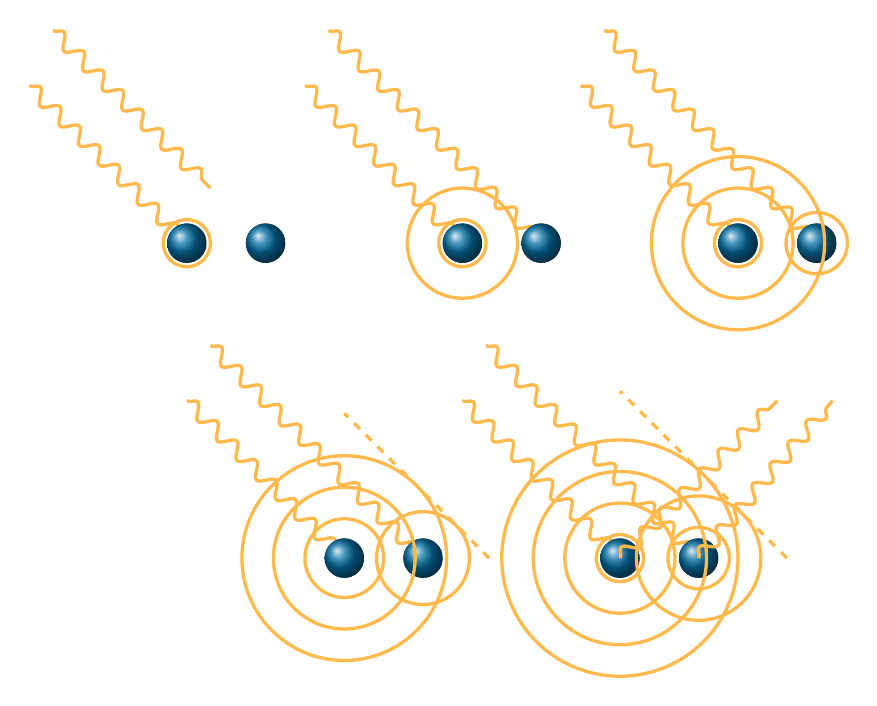
\begin{tikzpicture}
            \tikzset{atom/.style = {ball color=highlight, very thick}}
            \tikzset{wave/.style={complementary, very thick, decoration=snake, decorate}}
            \tikzset{circ/.style={complementary, very thick}}
            \draw[wave] (-2, 2) -- (0, 0);
            \draw[wave] (-1.7, 2.7) -- (0.3, 0.7);
            \fill[atom] (0, 0) circle [radius = 0.25];
            \fill[atom] (1, 0) circle [radius = 0.25];
            \draw[circ] (0, 0) circle [radius = 0.3];
            \begin{scope}[xshift=3.5cm]
                \draw[wave] (-2, 2) -- (0, 0);
                \draw[wave] (-1.7, 2.7) -- (1, 0);
                \fill[atom] (0, 0) circle [radius = 0.25];
                \fill[atom] (1, 0) circle [radius = 0.25];
                \draw[circ] (0, 0) circle [radius = 0.7];
                \draw[circ] (0, 0) circle [radius = 0.3];
            \end{scope}
            \begin{scope}[xshift=7cm]
                \draw[wave] (-2, 2) -- (0, 0);
                \draw[wave] (-1.7, 2.7) -- (1, 0);
                \fill[atom] (0, 0) circle [radius = 0.25];
                \fill[atom] (1, 0) circle [radius = 0.25];
                \draw[circ] (0, 0) circle [radius = 1.1];
                \draw[circ] (0, 0) circle [radius = 0.7];
                \draw[circ] (0, 0) circle [radius = 0.3];
                \draw[circ] (1, 0) circle [radius = 0.39];
            \end{scope}
            \begin{scope}[xshift=2cm, yshift=-4cm]
                \draw[wave] (-2, 2) -- (0, 0);
                \draw[wave] (-1.7, 2.7) -- (1, 0);
                \fill[atom] (0, 0) circle [radius = 0.25];
                \fill[atom] (1, 0) circle [radius = 0.25];
                \draw[circ] (0, 0) circle [radius = 1.3];
                \draw[circ] (0, 0) circle [radius = 0.9];
                \draw[circ] (0, 0) circle [radius = 0.5];
                \draw[circ] (1, 0) circle [radius = 0.59];
                \draw[dashed, circ] (1.84, 0) -- (0, 1.84);
            \end{scope}
            \begin{scope}[xshift=5.5cm, yshift=-4cm]
                \draw[wave] (-2, 2) -- (0, 0);
                \draw[wave] (-1.7, 2.7) -- (1, 0);
                \fill[atom] (0, 0) circle [radius = 0.25];
                \fill[atom] (1, 0) circle [radius = 0.25];
                \draw[circ] (0, 0) circle [radius = 1.5];
                \draw[circ] (0, 0) circle [radius = 1.1];
                \draw[circ] (0, 0) circle [radius = 0.7];
                \draw[circ] (0, 0) circle [radius = 0.3];
                \draw[circ] (1, 0) circle [radius = 0.79];
                \draw[circ] (1, 0) circle [radius = 0.39];
                \draw[dashed, circ] (2.12, 0) -- (0, 2.12);
                \draw[wave] (0, 0) -- (2, 2);
                \draw[wave] (1, 0) -- (2.7, 2);
            \end{scope}
        \end{tikzpicture}
        \caption{Two atoms in a crystal absorb and re-emit light.}
    \end{figure}

    \subsection{Bragg's Law}
    \defineindex{Bragg's law} states that for interplanar spacing \(d_{hk\ell}\) and radiation wavelength \(\lambda\) there will be constructive interference at angle \(2\vartheta\) if
    \begin{equation}
        2d_{hk\ell} \sin\vartheta = \lambda
    \end{equation}
    This is the crystallographer's version of Bragg's law, normally there is a factor of \(n \in \integers\) but this isn't needed when we consider whole families of planes at a time.
    
    Bragg's derivation of this law assumes that the crystal planes act like perfect mirrors.
    Further, this law gives us no information about the diffracted intensities and cannot account for systematic absences.
    
    Bragg's law does allow us to determine the unit cell dimensions and hence the lattice part of the crystal structure.
    What it can't do is tell us anything about the arrangement of atoms in this lattice, i.e. the crystal basis.
    For this we will need a fuller description of the diffraction process.
    
    \subsection{The Maths of Diffraction}
    Suppose the incident light is an electromagnetic plane wave with wave vector \(\vv{k}\), that is proportional to \(\e^{i\vv{k}\cdot\vv{r}}\).
    Similarly the diffracted beam is an electromagnetic plane wave with wave vector \(\vv{k'}\), and hence proportional to \(\e^{i\vv{k'}\cdot\vv{r}}\).
    
    We now that \(\abs{\vv{k}} = 2\pi/\lambda\), where \(\lambda\) is the wavelength of the radiation.
    The phase of the wave at \(\vv{r}\) is given by \(\vv{k}\cdot\vv{r}\).
    In a diffraction process there is no change in wavelength and so \(\abs{\vv{k}} = \abs{\vv{k'}} = k\).
    This assumes elastic scattering, meaning the total energy is constant, and since \(E = \hbar c k\) this means \(k\) is constant.
    This is a reasonable assumption as any effects due to inelastic scattering are necessarily weaker due to loss of energy.
    
    Assuming x-ray diffraction the diffraction occurs due to interaction with the electrons.
    We can describe the positions of the electrons with the electron density, \(n(\vv{r})\).
    
    We consider the phase shift at each point in the crystal.
    The phase shift at some point \(\vv{r}\) is \((\vv{k} - \vv{k'})\cdot\vv{r}\).
    We can account for the phase shift from each point of the crystal by integrating over the volume of the crystal.
    This gives us the \defineindex{scattering amplitude}:
    \begin{equation}
        F(\vv{k}, \vv{k'}) = \int\limits_{\text{crystal}} n(\vv{r}) \exp[i (\vv{k} - \vv{k'}) \cdot \vv{r}] \dd{V}.
    \end{equation}
    This measures the strength of diffraction of a wave entering in the direction \(\vh{k}\) and exiting in the direction \(\vh{k}\vv{'}\).
    
    For periodic crystals \(n(\vv{r})\) is periodic in space.
    This suggests that we should use Fourier series.
    
    \subsection{Fourier Series Recap}
    \subsubsection{One Dimension}
    A function is periodic if \(n(x + a) = n(x)\) for all \(x\) for some specific value of \(a\).
    We call \(a\) the period of the function.
    A periodic function can be expanded as a Fourier series.
    In the one-dimensional case the function \(n\) can be expanded as
    \begin{equation}
        n(x) = \frac{1}{2} C_0 + \sum_{p=1}^{\infty} \left[ C_p \cos\left( \frac{1\pi p x}{a} \right) + S_p \sin \left( \frac{2\pi p x}{a} \right) \right].
    \end{equation}
    The coefficients are given by
    \begin{align}
        C_p &= \frac{2}{a} \int_0^a n(x) \cos\left( \frac{2\pi px}{a} \right) \dd{x},\\
        S_p &= \frac{2}{a} \int_0^a n(x) \sin\left( \frac{2\pi px}{a} \right) \dd{x}.
    \end{align}
    
    We can similarly expand \(n\) in a complex Fourier series:
    \begin{equation}
        n(x) = \sum_{p=-\infty}^{\infty} n_p \e^{2\pi i px/a}
    \end{equation}
    where
    \begin{equation}
        n_p = \frac{1}{a}\int_0^a n(x) \e^{-2\pi i px/a}\dd{x}.
    \end{equation}
    If \(n\) is a real function then \(n_{-p} = n_p^*\).
    
    Notice that if \(x\) is a length then \(p\) has units of inverse length.
    
    \subsubsection{Higher Dimensions}
    In two or more dimensions we can do something similar.
    Consider a two-dimensional function \(n\) which is periodic in both of its inputs.
    Then the Fourier series of this function follows very easily from the one dimensional case:
    \begin{equation}
        n(x, y) = \sum_{p, q = -\infty}^{\infty} n_{p,q}\e^{2\pi i px/a}\e^{2\pi i qy/b}
    \end{equation}
    where \(a\) is the period along the \(x\)-axis and \(b\) is the period along the \(y\)-axis.
    An example may be a primitive rectangular lattice with lattice parameters \(a\) and \(b\) where \(n\) is the electron density treating the atoms as points.
    We can define a \defineindex{reciprocal lattice} made of the points
    \begin{equation}
        (2\pi \frac{px}{a}, 2\pi\frac{qy}{b})
    \end{equation}
    for \(p, q \in \integers\).
    
    For a crystal that isn't periodic in the same way we cannot use a Fourier series quite so easily.
    Instead we define a lattice in reciprocal space.
    We define
    \begin{align}
        \vv{a_1^*} &= 2\pi \frac{\vv{a_2}\times\vv{a_3}}{\vv{a_1}\cdot(\vv{a_2}\times\vv{a_3})} = \frac{2\pi}{V} \vv{a_2}\times\vv{a_3},\\
        \vv{a_2^*} &= 2\pi \frac{\vv{a_3}\times\vv{a_1}}{\vv{a_2}\cdot(\vv{a_3}\times\vv{a_1})} = \frac{2\pi}{V} \vv{a_3}\times\vv{a_2},\\
        \vv{a_3^*} &= 2\pi \frac{\vv{a_1}\times\vv{a_2}}{\vv{a_3}\cdot(\vv{a_1}\times\vv{a_2})} = \frac{2\pi}{V} \vv{a_1}\times\vv{a_2}.
    \end{align}
    These are called the \defineindex{reciprocal lattice vectors}.
    We then form a lattice from the points
    \begin{equation}
        \vv{G} = v_1\vv{a_1^*} + v_2\vv{a_2^*} + v_3\vv{a_3^*}
    \end{equation}
    with \(v_i \in \integers\).
    
    Notice that from this definition
    \begin{equation}
        \vv{a_i^*} \cdot \vv{a_j} = 2\pi \delta_{ij}.
    \end{equation}
    
    We call the space described by \(\vv{a_i}\) \enquote{real space}, \enquote{crystal space}, or \enquote{direct space}, and the space described by \(\vv{a_i^*}\) \enquote{reciprocal space}.
    
    Reciprocal lattice vectors have units of inverse length.
    
    \begin{ntn}{Lattice Vector Conventions}{}
        There are a few common conventions for what lattice vectors, and reciprocal lattice vectors, are called:
        \begin{tabular}{ll}\toprule
            \multicolumn{2}{c}{This course}\\
            Real space: & \(\vv{a_1}\), \(\vv{a_2}\), \(\vv{a_3}\)\\
            Reciprocal space: & \(\vv{a_1^*}\), \(\vv{a_2^*}\), \(\vv{a_3^*}\)\\\midrule
            \multicolumn{2}{c}{Kittel (textbook)}\\
            Real space: & \(\vv{a_1}\), \(\vv{a_2}\), \(\vv{a_3}\)\\
            Reciprocal space: & \(\vv{b_1}\), \(\vv{b_2}\), \(\vv{b_3}\)\\\midrule
            \multicolumn{2}{c}{Crystallographer}\\
            Real space: & \(\vv{a}\), \(\vv{b}\), \(\vv{c}\)\\
            Reciprocal space: & \(\vv{a*}\), \(\vv{b^*}\), \(\vv{c^*}\)\\\bottomrule
        \end{tabular}
    \end{ntn}

    Every crystal therefore has two attached lattices.
    First, the real-space lattice, in which translation vectors, \(\vv{a_i}\), have dimensions of length.
    This lattice tells us abut the periodicity of the atomic arrangement.
    Second, the reciprocal lattice, in which translation vectors, \(\vv{a_i^*}\), have dimensions of inverse length.
    This lattice is a lattice in Fourier space and is useful for dealing with periodic functions, such as charge density, and scattering processes.
    
    All non-centred lattices have the same form in reciprocal space, for example a cubic lattice will have a cubic reciprocal lattice.
    Centred lattices aren't so simple.
    
    We can use the reciprocal lattice to define a Fourier series expansion for \(n(\vv{r})\):
    \begin{equation}
        n(\vv{r}) = \sum_{\vv{G}} = n_{\vv{G}} \e^{i\vv{G}\cdot\vv{r}}
    \end{equation}
    where \(\vv{G} = v_1\vv{a_1^*} + v_2\vv{a_2^*} + v_3\vv{a_3^*}\) with \(v_i\in\integers\).
    The Fourier coefficients are given by
    \begin{equation}
        n_{\vv{G}} = \frac{1}{V_{\text{cell}}} \int_{\mathrlap{\text{unit cell}}} \,n(\vv{r}) \e^{-i\vv{G}\cdot\vv{r}}\dd{V}.
    \end{equation}
    Where \(V_\mathrm{cell}\) is the volume of the unit cell.
    
    \section{The Lattice Vector}
    The reciprocal lattice vector
    \begin{equation}
        \vv{G^*} = h\vv{a_1^*} + k\vv{a_2^*} + \ell\vv{a_3^*}
    \end{equation}
    is perpendicular to the \(\crystalplane{h}{k}{\ell}\) plane.
    To see that this is true we use the fact that this plane intercepts the axes at \(\vv{a_1}/h\), \(\vv{a_2}/k\), and \(\vv{a_3}/\ell\).
    This gives us two vectors \(\vv{a_1}/h - \vv{a_2}/k\) and \(\vv{a_1}/h - \vv{a_3}/\ell\) which are in the plane.
    We can then dot these with \(\vv{G^*}\) and we see we get zero both times.
    This result holds for \emph{all} types of crystals.
    The earlier result that \(h\vv{a_1} + k\vv{a_2} + \ell\vv{a_3}\) is perpendicular to the plane only holds for orthorhombic crystals where all angles are right angles.
    
    The interplanar spacing, \(d_{hk\ell}\), is given by
    \begin{equation}
        d_{hk\ell} = \frac{2\pi}{\abs{\vv{G^*}}}.
    \end{equation}
    To show this is true we we notice that consecutive planes cross the \(\vv{a_1}\) axis at \(\vv{a_1}/h\) and \(2\vv{a_1}/h\) and we use the formula \(\vh{n}\cdot\vv{r} = d\), which gives the distance, \(d\), from the origin for a plane with unit normal \(\vh{n}\) containing the point \(\vv{r}\).
    In our case we use \(\vv{r}\) as the points \(\vv{a_1}/h\), and \(2\vv{a_1}/h\) and \(\vh{n} = \vv{G^*}/\abs{\vv{G^*}}\).
    We then work out the two values of \(d\) and the difference of these is the interplanar spacing.
    This works for \emph{all} types of crystals.
    
    For the special case of orthorhombic crystals (all angles right angles) we can simplify this relationship to get
    \begin{equation}
        \frac{1}{d_{hk\ell}} = \sqrt{\frac{h^2}{a^2} + \frac{k^2}{b^2} + \frac{\ell^2}{c^2}}.
    \end{equation}
    For a cubic crystal (also all sides equal) this simplifies further to
    \begin{equation}
        \frac{1}{d_{hk\ell}} = \sqrt{\frac{h^2 + k^2 + \ell^2}{a^2}}.
    \end{equation}
    
    \section{Diffraction Intensities}
    We shall focus on x-ray diffraction as the most common case but similar work should apply to other types of diffraction.
    In x-ray diffraction electrons absorb x-rays and oscillate.
    They then emit x-rays in all directions (although not with equal intensity).
    We assume that the electron density distribution, \(n(\vv{r})\), is known for a given crystal.
    We then integrate over all contributions to the emitted radiation, accounting for phase differences.
    We will find that most cases cancel out leaving us with only a few diffraction angles at which we get bright spots.
    
    We said previously that the scattering amplitude is
    \begin{equation}
        F(\vv{k}, \vv{k'}) = \int\limits_{\text{crystal}} n(\vv{r})\exp[i(\vv{k} - \vv{k'})\cdot\vv{r}]\dd{V}.
    \end{equation}
    Introducing the \defineindex{scattering vector} \(\vv{\Delta k}\), sometimes denoted \(\vv{Q}\) instead, this becomes
    \begin{equation}
        F_{\vv{\Delta k}} = \int\limits_{\text{crystal}} n(\vv{r}) \e^{-i\vv{\Delta k}\cdot\vv{r}}\dd{V}.
    \end{equation}
    We can recognise this as simply the Fourier transform of the electron density, \(n(\vv{r})\).
    
    Inserting the Fourier expansion of \(n(\vv{r})\) we have
    \begin{align}
        F_{\vv{\Delta k}} &= \int\limits_{\text{crystal}} \sum_{\vv{G}} n_{\vv{G}} \e^{-(\vv{G} - \vv{\Delta k})\cdot\vv{r}}\dd{V}\\
        \sum_{\vv{G}} n_{\vv{G}} \int\limits_{\text{crystal}} \e^{-[\vv{G} - \vv{\Delta k}]\cdot\vv{r}}
    \end{align}
    where we have assumed that the Fourier series converges uniformly and so swapping the sum and integral is valid\footnote{all reasonable physical functions, including the electron density, are smooth enough for uniform convergence of their Fourier series}.
    
    Suppose that \(\vv{G} = \vv{\Delta k}\) for some specific \(\vv{G}\).
    Then for this term in the series we have
    \begin{equation}
        n_{\vv{G}} \int\limits_{\text{crystal}} \dd{V} = n_{\vv{G}}V
    \end{equation}
    where \(V\) is the volume of the crystal.
    
    Now suppose \(\vv{G} \ne \vv{\Delta k}\).
    We then have that \(\abs{\vv{G} - \vv{\Delta k}} \approx 2\pi/\qty{1}{\angstrom} \approx \qty{e11}{m^{-1}}\) and for a typical crystal size of a few millimetres we have \(\abs{\vv{r}} \approx \qty{1}{\milli\meter} \approx \qty{e-3}{\meter}\).
    Hence we find that \(\abs{(\vv{G} - \vv{\Delta k})\cdot\vv{r}} \approx \num{e8}\).
    This is huge.
    The complex exponential factor is then rapidly oscillating.
    The result is that over the entire integral these oscillations cancel out and we get zero.
    
    Combing these two results we have
    \begin{equation}
        F_{\vv{\Delta k}} = 
        \begin{cases}
            n_{\vv{G}}V, &\text{if }\vv{\Delta k} = \vv{G}\text{ for some specific }\vv{G},\\
            0, &\text{else}.
        \end{cases}
    \end{equation}
    As a result we only consider the case when \(\vv{\Delta k} = \vv{G}\) for some \(\vv{G} = h\vv{a_1^*} + k\vv{a_2^*} + \ell\vv{a_3^*}\), which means we only consider \(F_{\vv{G}}\), or in alternative notation \(F_{hk\ell}\).
    This gives rise to the \defineindex{Laue diffraction condition} that \(F_{\vv{\Delta k}} \ne 0\) only if \(\vv{\Delta k} = \vv{G}\).
    
    The diffraction intensity from the plane \(\crystalplane{h}{k}{\ell}\) is \(I_{hk\ell}\) and this is proportional to \(\abs{F_{hk\ell}}^2 = \abs{F_{\vv{G}}}^2 \propto \abs{n_{\vv{G}}}\).
    
    There is an equivalent ways to state the Laue diffraction condition.
    First, rearranging the condition that \(\vv{G} = \vv{\Delta k} = \vv{k'} - \vv{k}\) we have \(\vv{k'} = \vv{k} + \vv{G}\) and so
    \begin{equation}
        \vv{k'}\cdot\vv{k'} = (\vv{k} + \vv{G})\cdot(\vv{k} + \vv{G}) \implies \abs{\vv{k'}}^2 = \abs{\vv{k}}^2 + 2\vv{k}\cdot\vv{G} + \abs{\vv{G}}^2.
    \end{equation}
    This gives \(-2\vv{k}\cdot\vv{G} = \abs{\vv{G}}^2\) since \(\abs{\vv{k}} = \abs{\vv{k'}}\) for elastic scattering.
    WE can then consider a reciprocal lattice vector \(\vv{G'} = -\vv{G}\) in which case we have \(2\vv{k}\cdot\vv{G'} = \abs{\vv{G'}}^2 = G^2\) noticing that \(\vv{G}\) and \(\vv{G'}\) are equivalent when we sum over all lattice vectors we can simply call \(\vv{G'}\) \(\vv{G}\) and we have the condition
    \begin{equation}
        \vv{k}\cdot\vv{G} = \frac{1}{2}\abs{\vv{G}}^2.
    \end{equation}

    From this we can define \(\vartheta_{hk\ell}\) as the angle between \(\vv{k}\) and \(\vv{G}\) and we have
    \begin{equation}
        \vv{k}\cdot\vv{G} = kG\sin\vartheta_{hk\ell} = \frac{1}{2}\abs{\vv{G}}^2 = \frac{1}{2}\left( \frac{2\pi}{d_{hk\ell}} \right)^2.
    \end{equation}
    Noticing that \(k = 2\pi/\lambda\) and \(G = 2\pi/d_{hkl}\) this becomes
    \begin{equation}
        2d_{hk\ell}\sin\vartheta_{hk\ell} = \lambda
    \end{equation}
    and so we have derived \defineindex{Bragg's law} without resorting to assumptions of specular reflection.
    
    \section{Form Factors}
    The diffraction intensity, \(I_{hk\ell}\), is proportional to the magnitude squared of the Fourier coefficients of the electron density.
    Therefore we don't have enough information from the diffraction intensity to recover the Fourier coefficients, and hence to recover the electron density.
    
    In the case when we do have diffraction, i.e. \(\vv{\Delta k} = \vv{G}\), we have the scattering amplitude
    \begin{equation}
        F_{\vv{G}} = \int\limits_{\text{crystal}} n(\vv{r})\e^{-i\vv{G}\cdot\vv{r}}\dd{V}.
    \end{equation}
    If our crystal consists of \(N\) unit cells then this is 
    \begin{equation}
        F_{\vv{G}} = N\int\limits_{\mathrlap{\text{unit cell}}} n(\vv{r})\e^{-i\vv{G}\cdot\vv{r}}\dd{V}.
    \end{equation}
    
    We can approximate \(n(\vv{r})\) as a superposition of free-atom electron densities by neglecting the few electrons that take part in the chemical bonding.
    Doing so and summing over the \(s\) atoms in the unit cell we have
    \begin{equation}
        n(\vv{r}) \approx \sum_{j=1}^{s} n_j(\vv{r} - \vv{r_j})
    \end{equation}
    where \(n_j(\vv{\rho})\) is the free-atom electron density of the \(j\)th atom with \(\vv{\rho}\) being the position taking the centre of the atom, \(\vv{r_j}\), to be the origin.
    
    We can define the \defineindex{atomic form factor}, \(f_j(G)\), to be
    \begin{equation}
        f_j(G) \coloneqq \int n_j(\vv{\rho}) \e^{-i\vv{G}\cdot\vv{\rho}}\dd{V}
    \end{equation}
    where we note that the spherical symmetry of atoms means this is a function of \(G\) rather than \(\vv{G}\).
    The Fourier coefficients are then given by
    \begin{equation}
        F_{\vv{G}} = N\sum_{j=1}^{s} f_j(G)\e^{-i\vv{G}\cdot\vv{r_j}}.
    \end{equation}
    
    In practice it isn't possible to know the exact number of unit cells present in a crystal sample, and we don't need to since we are only interested in proportionality.
    We then define the \defineindex{structure factor}
    \begin{equation}
        S_{hk\ell} = S_{\vv{G}} = \sum_{j=1}^{s} f_j(G)\e^{-i\vv{G}\cdot\vv{r_j}} = \sum_{j} f_j \exp[-2\pi i(hx_j + ky_j + \ell z_j)]
    \end{equation}
    where we take \(\vv{r_j} = x_j\vv{a_1} + y_j\vv{a_2} + z_j\vv{a_3}\) and \(\vv{G} = h\vv{a_1^*} + k\vv{a_2^*} + \ell\vv{a_3^*}\) and used \(\vv{a_i^*}\cdot\vv{a_j} = 2\pi\delta_{ij}\).
    
    It is the structure factor with which we work when considering diffraction.
    We know that
    \begin{equation}
        I_{hk\ell} \propto \abs{S_{hk\ell}}^2
    \end{equation}
    and so we lose information about phase.
    This means that we can't work backwards to find the electron density but this is enough to rule out many crystal structures that are completely wrong.
    
    \section{Diffraction Techniques}
    \subsection{Laue Diffraction}
    Laue diffraction was the original technique for x-ray crystallography.
    In this process \enquote{white} (meaning a range of wavelengths) broadband spectrum x-rays are used.
    A single crystal is used as a sample and is placed in the x-ray beam.
    The diffracted x-rays are collected using some sort of sensor all at once.
    
    This method is best suited to simple crystals, in particular it is often used to ascertain the orientation of a crystal before a more sensitive experiment.
    It is difficult to model the exact intensities of diffraction due to the range of wavelengths.
    
    \subsection{Monochromatic Single Crystal Diffraction}
    This is the modern standard for x-ray crystallography.
    A single crystal is placed in a beam of monochromatic (single wavelength) x-rays.
    The diffracted x-rays are collected as the sample is rotated.
    At any one time x-rays are only diffracted to a few points but by rotating the sample a larger picture can be built up.
    The result is a picture which is mostly dark but with a few bright spots.
    From this it is possible to work out which planes caused the diffraction and from the relative intensities we can measure the magnitude of the structure factor.
    
    For less sensitive work x-ray tubes can produce the required x-ray beams.
    More sensitive work requiring higher energy, more focused beams often uses synchrotron radiation.
    
    \subsection{Monochromatic Powdered Crystal Diffraction}
    Often it is not possible to come up with a single crystal large enough for the procedure in the previous section.
    Instead a polycrystalline powder can be used.
    The setup is otherwise identical.
    Since the crystals in the powder are arranged randomly it is not necessary to rotate the sample.
    A single image can be captured.
    The result will be a series of rings as the crystals diffract in random directions but always at the same angle.
    Integrating around the rings gives the relative intensity, it is not enough to consider the intensity at a point on the ring due to the varying size of the rings.
    It should be possible to assign to each ring the plane from which the diffraction occurred.
    
    \subsection{Atomic Form Factor}
    Diffraction experiments, particularly powder diffraction, will show an overall decrease in intensity with increasing diffraction angle.
    Partly this is geometric, at larger angles the rings are larger and so the same intensity would be spread over a larger area.
    However, the effect remains when taking this into account.
    
    A second factor is destructive interference of x-rays scattered from different parts of the same atom.
    The atomic form factor is the Fourier transform of the charge distribution.
    It describes the interference of waves scattered from different parts of the same atom.
    When we consider x-rays the atomic form factor \(f(0)\) gives the number of electrons in the atom, which can be seen from
    \begin{equation}
        f(0) = \int n(\vv{\rho}) \e^{0} \dd{V}.
    \end{equation}
    Here \(\vv{\rho}\) is the distance from the centre of the atom.
    
    If we take the atoms to be point like scatterers, which is almost the case for neutron diffraction, then the atomic form factors reduce to a constant.
    
    The atomic form factor is a function of \(G\), which, combining Bragg's law and \(d = 2\pi/G\) is given by \(G = 4\pi\sin(\vartheta)/\lambda\).
    The values \(f(\sin(\vartheta)/\lambda)\) are tabulated for all elements.
    
    \subsection{Neutron Diffraction}
    The data produced by neutron diffraction is very similar to that produced by x-ray diffraction.
    The main difference being that x-rays are scattered by the extended electron cloud whereas neutrons are scattered by the nucleus, which is essentially a point particle.
    This results in atomic form factors which are independent of the scattering angle.
    We call these form factors the neutron scattering length.
    The result is that neutrons scattering doesn't have the same drop off with diffraction angle.
    
    Neutrons are generally produced in one of two ways.
    The more old fashioned way is from nuclear reactors.
    More modern setups us spallation sources, which is a fancy way of saying we smash protons into targets at high energy to produce neutrons.
    One issue with neutron diffraction is that neutrons are neutral and therefore we can't use magnetic fields to accelerate them and focus beams in the same way we do with other particles.
    
    \section{Systematic Absences}
    After a diffraction experiment if we have successfully assigned planes to all data points we may see that some planes don't appear.
    These are called \define{systematic absences}\index{systematic absence}.
    These are a result of terms cancelling each other out due to symmetry.
    This is best demonstrated with an example.
    
    \subsection{BCC Systematic Absences}
    Consider a BCC crystal.
    The structure factor is
    \begin{equation}
        S_{hk\ell} = S_{\vv{G}} = \sum_j f_j \e^{-2\pi i(hx_j + ky_j + \ell z_j)}.
    \end{equation}
    We consider the conventional cubic lattice, not the primitive lattice.
    The lattice vectors are \(\vv{a_i} = a\ve{i}\).
    The basis has atoms positioned at \(\vv{r_1} = (0, 0, 0)\), and \(\vv{r_2} = (1/2, 1/2, 1/2)\).
    There is only one type of atom in this simple example and so \(f_1 = f_2 = f\).
    Putting this into the formula for the structure factor we have
    \begin{equation}
        S_{hk\ell} = f[\e^{-2\pi i(0)} + \e^{=2\pi i (h + k + \ell)/2}] = f[1 + \e^{i\pi(h + k + \ell)}].
    \end{equation}
    We see that when \(h + k + \ell\) is odd the second exponential gives \(-1\) and therefore the structure factor is zero:
    \begin{equation}
        S_{hk\ell} = 
        \begin{cases}
            2f, & h + k + \ell \text{ even},\\
            0 & h + k + \ell \text{ odd}.
        \end{cases}
    \end{equation}
    So there is a systematic absence when \(h + k + \ell\) is odd.
    
    We can see this as a result of the symmetry of the crystal, hence why we cannot predict this effect from the lower symmetry primitive cell.
    We find a similar result for an FCC lattice:
    \begin{equation}
        S_{hk\ell} = 
        \begin{cases}
            2f, & \text{\(h\), \(k\), \(\ell\) all odd, or all even},\\
            0, & \text{else}.
        \end{cases}
    \end{equation}
    
    As another example in a C-centre lattice\footnote{recall that this is a lattice with a lattice point at the centre of the C face, that is the face spanned by \(\vv{a}\) and \(\vv{b}\).} we have a systematic absence when \(h + k\) is even.
    
    \section{FCC and BCC Reciprocal Lattices}
    Now that we are discussing diffraction from BCC and FCC crystals while we need to consider the reciprocal lattices for BCC and FCC.
    Recall that non-centred lattices are their own reciprocals, albeit with different lattice parameters.
    
    Consider the primitive cell for an FCC crystal.
    The primitive translation vectors are
    \begin{equation}
        \vv{a_1} = \frac{a}{2}(\vh{y} + \vh{z}), \qquad \vv{a_2} = \frac{a}{2}(\vh{z} + \vh{x}), \qqand \vv{a_3} = \frac{a}{2}(\vh{x} + \vh{y}).
    \end{equation}
    The volume of the primitive cell is
    \begin{equation}
        V = \abs{\vv{a_1} \cdot (\vv{a_2} \times \vv{a_3})} = \frac{1}{4}a^3.
    \end{equation}
    The reciprocal translation vectors are then given by
    \begin{equation}
        \vv{a_1^*} = \frac{2\pi}{V}\vv{a_2}\times\vv{a_3} = \frac{2\pi a^2}{4V}(\vh{x} + \vh{z}) \times (\vh{x} + \vh{y}) = \frac{2\pi}{a}(\vh{z} + \vh{y} - \vh{z})
    \end{equation}
    and similarly
    \begin{equation}
        \vv{a_2^*} = \frac{2\pi}{a}(\vh{x} + \vh{z} - \vh{y}), \qqand \vv{a_3^*} = \frac{2\pi}{a}(\vh{y} + \vh{x} - \vh{z}).
    \end{equation}
    These are simply the translation vectors for some BCC lattice in reciprocal space.
    We see that the reciprocal lattice for a FCC lattice is the BCC lattice, and since the reciprocal of the reciprocal is (up to a constant) the original lattice we know also that the reciprocal of a BCC lattice is the FCC lattice.
    
    \section{Diffraction Beyond Simple Systems}
    \subsection{DNA}
    Perhaps the most important example of x-ray diffraction on a complex system was the determination of the double-helix structure of DNA.
    This was discovered in experiments conducted by Rosalind Franklin.
    However, she was not fully recognised for this work at the time since she was a woman.
    She died before the Nobel prize was awarded to Francis Crick, James Watson, and Maurice Wilkins for their contributions to the discovery of the double helix and it is widely believed that had she been alive she would have been included in this prize.
    
    The key use of x-ray crystallography was to rule out a triple-helix structure that had been suggested.
    Like most x-ray crystallography it wasn't possible to confirm the double-helix structure through x-ray crystallography alone, but it could rule out competing hypotheses.
    
    \subsection{Small Angle Scattering}
    Small angle scattering is a technique used to obtain information about structures with characteristic length in the range \qtyrange{1}{100}{\nano\metre}.
    This covers structures from small viruses down to individual molecules.
    As the name suggests diffraction patterns at low angles, in the range \ang{0.1}--\ang{10}.
    Both x-rays and neutrons can be used, in which case the process is called small angle x-ray scattering (SAXS)\glossary[acronym]{SAXS}{small angle x-ray scattering} or small angle neutron scattering (SANS)\glossary[acronym]{SANS}{small angle neutron scattering}, respectively.
    One advantage of SANS is that neutrons interact more with hydrogen than x-rays do and for biological materials we are often interested in the location of hydrogen atoms.
    
    We saw with crystals that the atomic form factor plays an important role.
    This idea generalises to the notion of a form factor which encodes information about the size and shape of the object being studied.
    In small angle scattering it is conventional to work with the quantity \(Q = 4\pi\sin(\vartheta)/\lambda\), instead of the diffraction angle, \(2\vartheta\).
    
    \subsection{Aperiodic Crystals}
    So far we have only considered periodic crystals, and we will consider to do so for most of the course.
    We would be remiss, however, not to at least mention aperiodic crystals.
    
    It was initially believed that there are no crystals with five-fold symmetry.
    This is related to the idea that regular pentagons cannot tile the plane.
    However, (with the modern definition of crystals based on an essentially sharp diffraction pattern) there have been crystals discovered with 10-fold rotationally symmetric diffraction patterns, and therefore they also necessarily have five-fold rotational symmetry.
    The first example being a crystal made of zinc, magnesium and holmium.
    The existence of such a crystal is related to the ability to tile the plane aperiodically with five-fold symmetry, the most famous example using Penrose tiles.
    
    \begin{figure}
        \tikzsetnextfilename{penrose-tiling}
        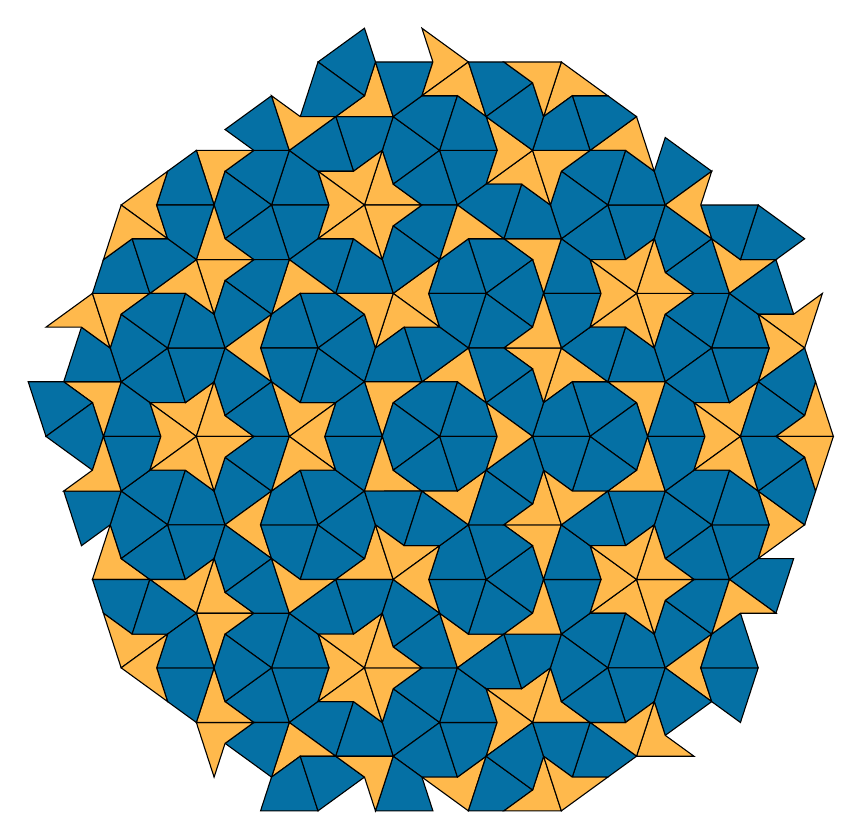
\begin{tikzpicture}[
                every Penrose tile/.style={draw},
                every kite/.style={fill=highlight},
                every dart/.style={fill=complementary}
            ]
            \foreach[evaluate=\k as \mk using {\k+Mod(\k,2)},evaluate=\k as
            \ax using {Mod(\k,2) == 0 ? "T" : "t"}] \k in {0,...,9} {
                \begin{scope}[rotate=\mk*36]
                    \PenroseDecomposition[Penrose step=5cm]{kite}{4}{\ax}
                \end{scope}
            }
        \end{tikzpicture}
        \caption{An aperiodic tiling of the plane with five-fold symmetry, known as a Penrose tiling.}
    \end{figure}
    
    Aperiodic crystals are often called \defineindex{quasicrystals}, since they don't fit earlier definitions of crystals.
    Since their first discovery many other examples have been found.
    
    \chapter{Crystal Binding}\label{sec:crystal binding}
    So far we've considered the shape of various crystals, but not why they form these shapes.
    To answer this we need to understand what holds crystals together.
    It's then a case of finding a minimum energy structure and over time a crystal will tend towards this form.
    There are four types of bonding that we need to consider.
    These are
    \begin{enumerate}
        \item Van der Waals' forces
        \item Ionic bonding
        \item Covalent bonding
        \item Metallic bonding
    \end{enumerate}
    Real crystals usually have a mixture of these.
    Van der Waals forces are the weakest and appear predominantly in noble gas crystals, since they are vastly overshadowed by any other bonding.
    Ionic bonds form between metals and non-metals when they exchange electrons to form ions which then attract each other.
    Covalent bonds form between non-metals when they share electrons, which they are both attracted to.
    Metallic bonds form, obviously, between metals where they lose electrons to form a sea of electrons and the resulting positive ions are then bound to this sea.
    
    When measuring bond strength force is not a very good measure since the force depends on the distance.
    Instead a better measure is the change in energy between a free system, with no interactions, and the system with interactions.
    A negative change in energy means that the interaction is attractive as the bound state is energetically favourable.
    On the other hand, a positive energy change means that the interaction is repulsive.
    
    Typically binding energies are
    \begin{enumerate}
        \item \(\sim\qty{0.1}{\electronvolt}\) per atom for rare gas crystals,
        \item \(\sim\qty{1}{\electronvolt} \) per atom for alkali metals,
        \item \(\sim\qtyrange{1}{10}{eV/atom}\) for other elemental crystals, and
        \item \(\sim\qtyrange{2}{6}{eV/atom}\) for ionic crystals.
    \end{enumerate}
    These are the \define{cohesive energies}\index{cohesive energy} of the crystals.
    They are defined as the energy required to form separated neutral atoms from the crystal.
    Precisely this requires moving the atoms infinitely far apart but in practice almost all of the energy is needed for just a small separation.
    
    \section{Van der Waals}
    \subsection{Attractive Component}
    The \defineindex{van der Waals} interaction is important in weakly bound crystals, such as noble-gas crystals, and also in soft matter, for example, when considering colloidal suspensions.
    They can even have microscopic effects, such as allowing Gecko's feet to stick to walls.
    Van der Waals interactions are present in all crystals but other interactions are much stronger if they are present.
    
    The mechanism behind the attractive component of the van der Waals interaction is instantaneous dipoles.
    In general we can model atoms as two charges, a positive charge fixed at a nucleus and a negative charge at the centre of the electron cloud.
    This negative charge is not stationary but moves around slightly due to random fluctuations in charge density.
    The charge separation results in an instantaneous dipole.
    If there is a nearby atom then this will induce in the atom a dipole aligned such that the two atoms attract each other.
    
    Of course this atom also has random fluctuations in charge density and so is forming its own instantaneous dipoles and interacting with its neighbours and so on.
    
    \subsubsection{Oscillator Model}
    We are interested in the attractive interaction between two dipoles.
    We can model these as quantum harmonic oscillators, see \cref{fig:dipole oscillators}.
    Each formed from two charges, \(\pm e\), which represent the charge of the nucleus and the valence electron.
    These are connected by a spring, which models the attraction between the charges.
    We fix the positive charges at some length \(R\), which is the nuclear separation.
    Each pair of charges is separated by \(x_i\).
    We want to know how the energy of the system changes as the dipoles are brought closer together.
    We will see that the solution is \(E \propto R^{-6}\).
    
    \begin{figure}
        \tikzsetnextfilename{double-dipole-oscillator}
        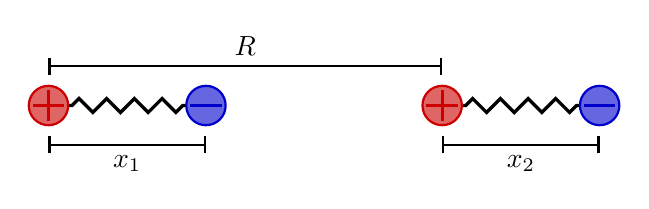
\begin{tikzpicture}
            \tikzset{charge/.style={draw, thick, #1, fill=#1!60, circle, minimum size=0.5cm, inner sep=0pt, font={\large}}}
            \tikzset{spring/.style={decoration={zigzag, pre length=0.3cm, post length=0.2cm}, decorate, very thick}}
            \draw[spring] (0, 0) -- (2, 0);
            \draw[spring] (5, 0) -- (7, 0);
            \node[charge=positive red] {};
            \node[charge=negative blue] at (2, 0) {};
            \node[charge=positive red] at (5, 0) {};
            \node[charge=negative blue] at (7, 0) {};
            \draw[positive red, very thick] (-0.2, 0) -- (0.2, 0);
            \draw[positive red, very thick] (0, -0.2) -- (0, 0.2);
            \draw[positive red, very thick] (4.8, 0) -- (5.2, 0);
            \draw[positive red, very thick] (5, -0.2) -- (5, 0.2);
            \draw[negative blue, very thick] (1.8, 0) -- (2.2, 0);
            \draw[negative blue, very thick] (6.8, 0) -- (7.2, 0);
            
            \draw[|-|, thick] (0, 0.5) -- (5, 0.5) node[midway, above] {\(R\)};
            \draw[|-|, thick] (0, -0.5) -- (2, -0.5) node[midway, below] {\(x_1\)};
            \draw[|-|, thick] (5, -0.5) -- (7, -0.5) node[midway, below] {\(x_2\)};
        \end{tikzpicture}
        \caption{The two dipole oscillators used to model van der Waals interactions.}
        \label{fig:dipole oscillators}
    \end{figure}
    
    We start by considering the unperturbed system.
    This is equivalent to considering the case of \(R = \infty\).
    The Hamiltonian for the unperturbed system is
    \begin{equation}
        \hamiltonian_0 = \frac{p_1^2}{2m} + \frac{1}{2}Cx_1^2 + \frac{p_2^2}{2m} + \frac{1}{2}Cx_2^2.
    \end{equation}
    This is simply the sum of the two independent oscillator's Hamiltonians.
    The natural frequency of these oscillators, \(\omega_0\), relates to the constant \(C\) by \(C = m\omega_0^2\).
    The energy of a single oscillator in the \(n\)th excited state is
    \begin{equation}
        E_n = \left( n + \frac{1}{2} \right) \hbar\omega_0
    \end{equation}
    with \(n \in \naturals\).
    It follows that the zero-point energy (ZPE)\glossary[acronym]{ZPE}{zero-point energy} of the two oscillator system is
    \begin{equation}
        E_0 = 2 \cdot\frac{1}{2}\hbar\omega_0.
    \end{equation}
    
    We can now add in a perturbation to the Hamiltonian corresponding to the interactions between the charges.
    The perturbation Hamiltonian is simply the sum of the Coulomb interactions between the pairs of charged particles:
    \begin{equation}
        \hamiltonian_1 = \frac{e^2}{R} + \frac{e^2}{R + x_1 - x_2} - \frac{e^2}{R + x_1} - \frac{e^2}{R - x_2}. \CGS
    \end{equation}

    \begin{rmk}
        This equation is in \defineindex{CGS} units, we will flag equations in CGS units with \CGSpic{} throughout.
        The CGS system of units uses centimetres, grams and seconds\glossary[acronym]{CGS}{centimetre, gram, second} as base units, as opposed to the SI\glossary[acronym]{SI}{syst\`eme international}, which uses metres, kilograms, and seconds.
        To convert this equation from CGS to SI replace \(e^2\) with \(e^2/(4\pi\varepsilon_0)\).
    \end{rmk}
    
    Returning to the problem at hand, this Hamiltonian is not easy to deal with.
    Assuming that \(\abs{x_1}, \abs{x_2} \ll R\) we can combine the terms over a common denominator and drop all but the highest order term.
    This leaves us with
    \begin{equation}
        \hamiltonian_1 \approx -\frac{2e^2x_1x_2}{R^3}.
    \end{equation}
    
    We can now consider the Hamiltonian for the full system:
    \begin{equation}
        \hamiltonian = \hamiltonian_0 + \hamiltonian_1 = \frac{p_1^2}{2m} + \frac{1}{2}Cx_1^2 + \frac{p_2^2}{2m} + \frac{1}{2}Cx_2^2 - \frac{2e^2x_1x_2}{R^3}.\CGS
    \end{equation}
    This is easiest to work with if we diagonalise.
    To do this we introduce a normal mode transformation defining
    \begin{equation}
        x_{\mathrm{s}} \coloneqq \frac{1}{\sqrt{2}}(x_1 + x_2), \qqand x_{\mathrm{a}} \coloneqq \frac{1}{\sqrt{2}}(x_1 - x_2).
    \end{equation}
    Similarly we define the momenta
    \begin{equation}
        p_{\mathrm{s}} \coloneqq \frac{1}{\sqrt{2}}(p_1 + p_2), \qqand p_{\mathrm{a}} \coloneqq \frac{1}{\sqrt{2}}(p_1 - p_2).
    \end{equation}
    We can rearrange these to find \(x_i\) and \(p_i\):
    \begin{align}
        x_1 &= \frac{1}{\sqrt{2}}(x_{\mathrm{s}} + x_{\mathrm{a}}), \qquad & x_2 &= \frac{1}{\sqrt{2}}(x_{\mathrm{s}} - x_{\mathrm{a}}),\\
        p_1 &= \frac{1}{\sqrt{2}}(p_{\mathrm{s}} + p_{\mathrm{a}}), \qquad & p_2 &= \frac{1}{\sqrt{2}}(p_{\mathrm{s}} - p_{\mathrm{a}}).
    \end{align}
    Substituting these into the Hamiltonian and simplifying gives
    \begin{equation}
        \hamiltonian = \frac{p_{\mathrm{s}}^2}{2m} + \frac{1}{2}\underbrace{\left( C - \frac{2e^2}{R^3} \right)}_{\eqqcolon m\omega_{\mathrm{s}}^2}x_{\mathrm{s}}^2 + \frac{p_{\mathrm{a}}^2}{2m} + \frac{1}{2}\underbrace{\left( C + \frac{2e^2}{R^3} \right)}_{\eqqcolon m\omega_{\mathrm{a}}^2}x_{\mathrm{a}}^2. \CGS
    \end{equation}

    We see that this is the sum of two independent oscillators with frequencies
    \begin{equation}
        \omega_{\mathrm{a}, \mathrm{s}} = \sqrt{\frac{1}{m}\left( C \pm \frac{2e^2}{R^3} \right)} = \omega_0 \sqrt{1 \pm \frac{2e^2}{CR^3}}. \CGS
    \end{equation}
    Using the Taylor expansion, \(\sqrt{1 + \varepsilon} \approx 1 + x/2 - x^2/8\), this becomes
    \begin{equation}
        \omega_{\mathrm{a}, \mathrm{s}} \approx \omega_0\left[ 1 \pm \frac{1}{2}\frac{2e^2}{CR^3} - \frac{1}{8}\left( \frac{2e^2}{CR^3} \right)^2 \right]. \CGS
    \end{equation}
    The total zero-point energy of the coupled system is then
    \begin{equation}
        E_0' = \frac{1}{2}\hbar\omega_{\mathrm{s}} + \frac{1}{2}\hbar\omega_{\mathrm{a}} = \hbar\omega_0\left[ 1 - \frac{1}{8}\left( \frac{2e^2}{CR^3} \right)^2 \right] = \hbar\omega_0\left( 1 - \frac{A}{R^6} \right) \CGS
    \end{equation}
    where
    \begin{equation}
        A = \frac{1}{8}\left( \frac{2e^2}{C} \right)^2. \CGS
    \end{equation}
    
    Recall that the zero point energy of the uncoupled system is \(E_0 = \hbar\omega_0\) and we see that the reduction in energy due to the coupling is
    \begin{equation}
        \Delta U = E_0' - E_0 = -\frac{A}{R^6}.
    \end{equation}
    This is negative and hence corresponds to an attractive interaction.
    The binding energy varies as \(R^{-6}\) and the attractive force,
    \begin{equation}
        F = -\diff{\Delta U}{R},
    \end{equation}
    varies as \(R^{-7}\).
    
    This attractive interaction depends on the zero-point energy of the system and hence is an inherently quantum effect.
    
    This interaction is known under a few names.
    We have been calling it the van der Waals interaction, after Johannes van der Waals, the experimentalist who discovered the effect.
    It is also sometimes called the \define{London interaction}\index{London interaction|see{van der Waals}}, after Fritz London, the theorist who first explained it.
    At the time of solving this problem London was working on the dispersion of light in glass and the relation of wave length and index of refraction, this can also be explained by the oscillator model of an atom.
    See the notes from the optics part of the Electromagnetism course.
    For this reason these are also sometimes called the \define{dispersion interaction}\index{dispersion interaction|see{van der Waals}}.
    The mechanism of inducing dipoles means that these are also called \define{induced dipole-dipole interactions}\index{induced dipole-dipole interaction|see{van der Waals}}.
    
    \subsection{Repulsive Term}
    The van der Waals interaction is entirely attractive.
    Yet, atoms don't all collapse to a single point.
    There must be some repulsive force we have not accounted for.
    It would not be unreasonable to assume that this comes from the Coulomb interaction between the positively charged nuclei.
    However, there is a far greater source of repulsion, from the Pauli exclusion principle.
    
    As the two nuclei are brought together their wave functions start to overlap.
    As a result the Pauli exclusion principle applies to \emph{all} electrons in the combined two-atom system.
    Assuming that both atoms start in their ground states the only way to combine the wave functions is to have some electrons become excited so that they aren't in the same state.
    This requires energy, meaning the potential energy increases, and hence the result is a repulsive force.
    
    To see an example of this consider combining two hydrogen atoms with their electrons both in the ground state, 1s, but with opposite spins.
    When combined we get a \ce{^2He} atom with two electrons, both in the ground state 1s and with opposite spins.
    The total electron energy is \qty{-78.98}{\electronvolt}.
    A similar situation with two electrons with aligned spins can only occur if upon merging one of the electrons is excited to 2s (note that the spin can't flip as we must conserve angular momentum).
    The total electron energy is then \qty{-59.38}{\electronvolt}.
    This is an increase in energy of \qty{-19.6}{\electronvolt}.
    For comparison in hydrogen the electron is only bound with \qty{-13.6}{\electronvolt} in its ground state.
    
    We can capture the essential features of this repulsive effect with an empirical potential.
    These are potentials which we use through no justification other than they work.
    One common potential is
    \begin{equation}
        U(R) = \lambda\e^{-R/\rho}
    \end{equation}
    where \(R\) is the internuclear separation, and \(\lambda\) and \(\rho\) are constants of some characteristic energy and length scale.
    A simpler potential which we will make use of is
    \begin{equation}
        U(r) = \frac{B}{R^{12}}
    \end{equation}
    where \(B\) is some constant.
    There is nothing particularly important about the exponent being 12.
    Models with \(R^{-10}\), for example, would work just as well with a different constant.
    The choice of 12 is mostly for computational efficiency, especially in the pre-computer days.
    Once we have calculated \(R^{-6}\) for the attractive component computing \(R^{-12}\) is as simple as squaring this result.
    
    \subsection{Lennard-Jones Potential}
    The \defineindex{Lennard-Jones potential} is the result of combining both the attractive and repulsive interactions.
    It is
    \begin{equation}
        U_{\LJ}(R) = 4\varepsilon\left[ \left( \frac{\sigma}{R} \right)^{12} - \left( \frac{\sigma}{R} \right)^{6} \right]
    \end{equation}
    where \(\varepsilon\) and \(\sigma\) are parameters related to the energy and length scale respectively.
    This describes the interaction between a \emph{single pair} of atoms.
    
    The minimum of the potential, that is the equilibrium interatomic distance for a diatomic Lennard-Jones molecule, is found by differentiation:
    \begin{align}
        0 &= \diff{U_{\LJ}}{R}[R=r_0]\\
        &= 4\varepsilon\left[ -12\frac{\sigma^{12}}{r_0^{13}} + 6\frac{\sigma^{6}}{r_0^{7}} \right]\\
        \implies 12\frac{\sigma^{12}}{r_0^{13}} &= 6\frac{\sigma^{6}}{r_0^{7}}\\
        \implies \frac{\sigma^{6}}{r_0^{6}} &= \frac{1}{2}\\
        \implies \frac{r_0}{\sigma} &= 2^{1/6} \approx 1.12246.
    \end{align}
    
    \section{Van der Waals Crystal}
    We now have the Lennard-Jones potential, describing the interaction between \emph{pairs} of atoms due to van der Waals interactions and the repulsive effect of Pauli's exclusion principle.
    To consider an entire crystal we need to consider all pairwise interactions between atoms.
    Start by numbering all atoms to give them names.
    We take some reference atom, \(i\), and we sum over all atoms, \(j\), apart from \(i\).
    For each term of the sum we calculate the potential, \(U_{\LJ}(r_{ij})\), where \(r_{ij}\) is the distance between atom \(i\) and atom \(j\).
    This calculates all pairwise interactions with atom \(i\).
    If we do this for every atom one at a time taking the role of the reference atom then the result will be \emph{twice} the total potential of the entire crystal.
    The result is two times too large since we have double counted the interaction between \(i\) and \(j\) and the interaction between \(j\) and \(i\).
    For this reason we add in a factor of \(1/2\).
    In maths the process we've just described is
    \begin{equation}
        U_{\tot} = \frac{1}{2}\sum_{i=1}^{N} \sum_{j\ne i} U_{\LJ}(r_{ij}).
    \end{equation}
    
    Assuming that \(N\) is large and the potential drops away with distance only the nearby atoms are important.
    The ordered nature of the crystal means that most atoms are in a similar configuration of nearby atoms.
    The exception is for atoms on or near the surface of the crystal.
    However, the number of surface atoms goes with the square of the crystal size and the number of interior atoms goes with the cube.
    Therefore for all but the smallest crystals we can treat the surface atoms as interior atoms and the error will be relatively small.
    The result is that each term of the sum over \(i\) is approximately the same and so we make the approximation
    \begin{equation}
        U_{\tot} = \frac{N}{2}\sum_{j\ne i} U_{\LJ}(r_{ij})
    \end{equation}
    where we now choose some random interior atom to be \(i\).
    
    Substituting in the full potential we have
    \begin{equation}
        U_{\tot} = \frac{N}{2}4\varepsilon \left[ \sum_{j\ne i}\left( \frac{\sigma}{r_{ij}} \right)^{12} - \sum_{j\ne i} \left( \frac{\sigma}{r_{ij}} \right)^{6} \right].
    \end{equation}
    We want to come up with a formula that we can apply to any lattice.
    For this reason we define \(r_{ij} = Rp_{ij}\) where \(R\) is the minimum interatomic spacing in the crystal, that is the nearest neighbour distance.
    This allows us to factor out the crystal-specific information from the sums leaving us with
    \begin{equation}
        U_{\tot}(R) = \frac{N}{2}4\varepsilon\bigg[ \left( \frac{\sigma}{R} \right)^{12} \underbrace{\sum_{j\ne i} \frac{1}{p_{ij}^{12}}}_{\eqqcolon a_{12}} - \left( \frac{\sigma}{R} \right)^6 \underbrace{\sum_{j\ne i} \frac{1}{p_{ij}^6}}_{\eqqcolon a_6} \bigg].
    \end{equation}
    Here we have defined the \defineindex{lattice sums}, \(a_6\) and \(a_{12}\):
    \begin{equation}
        a_{n} \coloneqq \sum_{j\ne i} \frac{1}{p_{ij}^n}.
    \end{equation}
    
    \subsection{Lattice Sums}
    \subsubsection{Two Dimensions}
    We will start with an example of a lattice sum in two dimensions, as these are easier to visualise.
    For geometrical simplicity we consider a square crystal.
    \Cref{fig:2d lattice sum} shows a reference atom and the distances to its five nearest neighbours.
    We can also count the number of nearest neighbours from this diagram.
    Since each nearest neighbour of a given order is the same distance from the reference atom we can combine the terms of the sum corresponding to the nearest neighbours.
    Going up to the fifth nearest neighbours we get have
    \begin{align}
        a_{12} &= \frac{4}{1^{12}} + \frac{4}{\sqrt{2}^{12}} + \frac{4}{2^{12}} + \frac{8}{\sqrt{5}^{12}} + \frac{4}{\sqrt{8}^{12}} + \dotsb\\
        &\approx 4 + 0.0625 + 0.000977 + 0.000512 + \dotsb\\
        &\approx 4.064.
    \end{align}
    
    \begin{figure}
        \tikzsetnextfilename{2d-lattice-sum}
        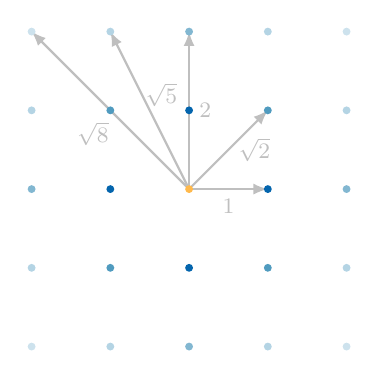
\begin{tikzpicture}
            \tikzset{lattice point/.style={inner sep=0pt, minimum size=0.1cm, circle}};
            \tikzset{arrow/.style={->, lightgray, thick, font={\footnotesize}}}
            \draw[arrow] (0, 0) -- (1, 0) node[midway, below] {\(1\)};
            \draw[arrow] (0, 0) -- (1, 1) node[midway, right] {\(\sqrt{2}\)};
            \draw[arrow] (0, 0) -- (0, 2) node[midway, right] {\(2\)};
            \draw[arrow] (0, 0) -- (-1, 2);
            \draw[arrow] (0, 0) -- (-2, 2);
            \node[lightgray, font={\footnotesize}] at (-0.35, 1.2) {\(\sqrt{5}\)};
            \node[lightgray, font={\footnotesize}] at (150:1.41) {\(\sqrt{8}\)};
            % Reference atom
            \node[lattice point, fill=complementary] at (0, 0) {};
            % 1st NN
            \node[lattice point, fill=highlight!90!blue] at (0, 1) {};
            \node[lattice point, fill=highlight!90!blue] at (0, -1) {};
            \node[lattice point, fill=highlight!90!blue] at (1, 0) {};
            \node[lattice point, fill=highlight!90!blue] at (-1, 0) {};
            % 2nd NN
            \node[lattice point, fill=highlight!70] at (1, 1) {};
            \node[lattice point, fill=highlight!70] at (1, -1) {};
            \node[lattice point, fill=highlight!70] at (-1, 1) {};
            \node[lattice point, fill=highlight!70] at (-1, -1) {};
            % 3rd NN
            \node[lattice point, fill=highlight!50] at (0, 2) {};
            \node[lattice point, fill=highlight!50] at (0, -2) {};
            \node[lattice point, fill=highlight!50] at (2, 0) {};
            \node[lattice point, fill=highlight!50] at (-2, 0) {};
            % 4th NN
            \node[lattice point, fill=highlight!30] at (2, 1) {};
            \node[lattice point, fill=highlight!30] at (2, -1) {};
            \node[lattice point, fill=highlight!30] at (-2, 1) {};
            \node[lattice point, fill=highlight!30] at (-2, -1) {};
            \node[lattice point, fill=highlight!30] at (1, 2) {};
            \node[lattice point, fill=highlight!30] at (1, -2) {};
            \node[lattice point, fill=highlight!30] at (-1, 2) {};
            \node[lattice point, fill=highlight!30] at (-1, -2) {};
            % 5th NN
            \node[lattice point, fill=highlight!20] at (2, 2) {};
            \node[lattice point, fill=highlight!20] at (2, -2) {};
            \node[lattice point, fill=highlight!20] at (-2, 2) {};
            \node[lattice point, fill=highlight!20] at (-2, -2) {};        \end{tikzpicture}
        \caption{A square crystal with distances from some reference atom.}
        \label{fig:2d lattice sum}
    \end{figure}
    
    From this we can see that the lattice sum is approximately the number of nearest neighbours with a small correction for the second nearest neighbours and an even smaller correction for the third nearest neighbours and so on.
    
    \subsubsection{Three Dimensions}
    A similar process can be applied to three-dimensional crystal structures, although the geometry is slightly more complicated.
    Again, we would find that each lattice sum is essentially the number of nearest neighbours with small corrections, although the corrections are slightly large than the two-dimensional case since the number of nearest neighbours goes with distance squared in the three-dimensional case but only with distance in the two-dimensional case.
    
    Fortunately people have already calculated the lattice sums for common lattices to far more precision than we could reasonably do.
    They found
    \begin{align}
        &\text{FCC:} \qquad & a_{12} &= 12.13188, \quad & a_{6} = 14.45392,\\
        &\text{HCP:} \qquad & a_{12} &= 12.13229, \quad & a_{6} = 14.45489,\\
        &\text{BCC:} \qquad & a_{12} &= 9.11418, \quad & a_{6} = 12.2533.
    \end{align}
    Notice that FCC and HCP have almost identical lattice sums.
    This is because the dominant effect in the lattice terms is the distance to nearest neighbours, which in turn is linked to the packing density, and the packing density of FCC and HCP is the same.
    It should also be noted that \(a_{12}\) is approximately the number of nearest neighbours, also known as the \defineindex{coordination number}.
    Both FCC and HCP have a coordination number of 12.
    BCC has a coordination number of 8.
    The discrepancy between \(a_{12} \approx 9.1\) and the coordination number 8 is due to the fact that the second nearest neighbours in a BCC crystal aren't that much further away than the nearest neighbours and therefore have a non-negligible contribution to the lattice sum.
    
    \subsection{Van der Waals Crystal Properties}
    Returning now to the potential we can find the equilibrium interatomic spacing in a crystal by finding the minimum of the potential:
    \begin{align}
        0 &= \diff{U_{\tot}}{R}[R=R_0]\\
        &= 2N\varepsilon\left[ -12a_{12}\frac{\sigma^{12}}{R_0^{13}} + 6a_6\frac{\sigma^{6}}{R_0^{7}} \right]\\
        \implies 12a_{12}\frac{\sigma^{12}}{R_0^{13}} &= 6a_6\frac{\sigma^{6}}{R_0^{7}}\\
        \implies \frac{\sigma^6}{R_0^6} &= \frac{a_{6}}{2a_{12}}\\
        \implies \frac{\sigma}{R_0} &= \left( \frac{a_6}{2a_{12}} \right)^{1/6}.
    \end{align}
    For comparison the interatomic spacing between two otherwise free atoms gave us \(r_0/\sigma = 2^{1/6} \approx 1.12\).
    For FCC and HCP we find that \(R_0/\sigma \approx 1.09\) and for BCC \(R_0/\sigma \approx 1.07\).
    We see that the interatomic spacing decreases slightly from the free diatomic molecule.
    
    In general the potential energy at equilibrium is
    \begin{equation}
        U_{\tot}(R_0) = 2N\varepsilon\left[ \left( \frac{a_6}{2a_{12}} \right)^{12} \right]a_{12} - \left( \frac{a_6}{2a_{12}} \right) = -4\varepsilon N\frac{a_6^2}{4a_{12}}.
    \end{equation}
    A more useful quantity is the binding energy per atom
    \begin{equation}
        U_0 = \frac{1}{N}U_{\tot}(R_0) = -4\varepsilon N\frac{a_6^2}{8a_{12}}.
    \end{equation}
    Evaluating this for FCC, HCP, and BCC crystals we find
    \begin{equation}
        \text{FCC:} \ -2.1525\cdot 4\varepsilon, \quad \text{HCP:} \ -2.1582\cdot 4\varepsilon, \qand \text{BCC:} \ -2.0592\cdot 4\varepsilon.
    \end{equation}
    From this we see that FCC and HCP are the most stable van der Waals crystals.
    The small difference between their binding energies per atom is negligible compared to approximations made in the derivation.
    
    This observation is born out in reality.
    When we cool the noble gases, \ce{Ne}, \ce{Ar}, \ce{Kr}, and \ce{Xe} down to a few kelvin they do indeed form FCC crystals.
    The lightest noble gas, \ce{He}, doesn't form a solid, even at absolute zero.
    This is because its zero-point energy is higher than the very small binding energy provided by van der Waals interactions.
    If we increase the pressure, essentially artificially decreasing interatomic spacing and hence increasing the strength of van der Waals interactions, then \ce{He} does form a crystal structure and this too agrees with our prediction that FCC and HCP are preferentially selected for by energy minimisation.
    
    \section{Ionic Binding}
    \subsection{Cohesive Energy}
    Recall that when we defined cohesive energy at the start of the chapter (\cref{sec:crystal binding}) we defined it as the energy required to separate a crystal into its \emph{neutral} constituent atoms.
    For an ionic crystal this means we need to consider not only the binding energy but also the energy required to create the ions from the neutral atoms.
    That is the ionisation energy for the positive ions and electron affinity for the negative ions.
    
    Consider, for example, \ce{NaCl}.
    This is formed from \ce{Na^+} ions and \ce{Cl^-} ions.
    We make the \ce{Na^+} ions in the reaction
    \begin{equation}
        \ce{Na_{\mathrm{g}}} + \text{Ionisation energy: \qty{5.14}{\electronvolt}} \longrightarrow \ce{Na^+_{\mathrm{g}}} + \Pe.
    \end{equation}
    Here the subscript \(\mathrm{g}\) denotes that we consider a gas of sodium atoms and ions, this is simply because this allows us to treat the interactions between atoms/ions as negligible.
    We make the \ce{Cl^-} ions in the reaction
    \begin{equation}
        \ce{Cl_{\mathrm{g}}} + \Pe \longrightarrow \ce{Cl^-_{\mathrm{g}}} + \text{Electron affinity: \qty{3.61}{\electronvolt}}.
    \end{equation}
    Note that both energies above are per atom/ion.
    We then form a single \ce{NaCl} unit in the reaction
    \begin{equation}
        \ce{Na^+_{\mathrm{g}}} + \ce{Cl^-_{\mathrm{g}}} \longrightarrow \ce{NaCl_{\mathrm{crystal}}} + \text{Binding energy: \qty{7.9}{\electronvolt}}.
    \end{equation}
    Combining these we see that when creating \ce{NaCl} from gaseous sodium and chlorine the energy change is
    \begin{equation}
        \qty{5.1}{\electronvolt} - \qty{3.6}{\electronvolt} - \qty{7.9}{\electronvolt} = -\qty{6.4}{\electronvolt}
    \end{equation}
    per \ce{NaCl} unit.
    Hence the cohesive energy of \ce{NaCl} is \qty{6.4}{\electronvolt} per \ce{NaCl} unit.
    We call this the energy per formula unit, sometimes abbreviated as \unit{\eVperFormulaUnit}.
    
    In reality in standard conditions chlorine forms a gas but sodium is in a metallic state.
    However, the cohesive energy of sodium metal is only \qty{1.1}{\eVperAtom}, and so creating \ce{NaCl} from the elements in their normal forms is still energetically favourable.
    
    One of the reasons that the ionic \ce{NaCl} is more stable than the elemental forms is that in the process of forming the ions both \ce{Na} and \ce{Cl} achieve full outer shells, \ce{Na} goes from \(\mathrm{[\ce{Ne}]3s}\) to \(\mathrm{[\ce{Ne}]}\), and \ce{Cl} goes from \(\mathrm{[\ce{Ne}]3s^23p^5}\) to \(\mathrm{[\ce{Ne}]3s^23p^6} = \mathrm{[\ce{Ar}]}\).
    These closed-shell configurations are very stable.
    It would require a large amount of energy to transfer more electrons, for example to create \ce{Na^{2+}} or \ce{Cl^{2-}}.
    
    \subsection{Ionic Crystals}
    We can now calculate the binding energy of an ionic crystal.
    The approach is similar to the van der Waals crystal but slightly complicated by having to consider two different ions with different charges.
    For simplicity we consider crystals formed of two ions of equal and opposite charge, this covers many, but not all, ionic crystals, for example this works for \ce{NaCl}, but not \ce{CaCl_2}.
    
    While all crystals, including ionic crystals, have van der Waals interactions they are very weak and so we ignore them in this case.
    
    Recall that the Pauli exclusion principle leads to a short-range repulsive force.
    We model this with an empirical potential, \(V_{\mathrm{r}}\), which we take to be \(V_{\mathrm{r}}(r) = \lambda\e^{-r/\rho}\), another common form is \(V_{\mathrm{r}}(r) = A/r^{n}\).
    We will leave the result in such a way that we can easily swap out different potentials.
    Further, we assume that this potential is short-range and we can ignore it between anything but nearest neighbours.
    
    The other interaction we have to consider is the long-range Coulomb interaction:
    \begin{equation}
        V_{\mathrm{C}}(r) = \pm \frac{q^2}{4\pi \varepsilon_0 r}.
    \end{equation}
    Here the ions have charge \(\pm q\), and the sign of \(\pm q^2\) depends on whether we consider a pair of atoms of equal or opposite charge.
    This potential decreases slowly with \(r\) (at least when compared to \(V_{\mathrm{r}}\)).
    In fact, \(V_{\mathrm{C}} \propto 1/r\).
    The number of \(k\)-nearest neighbours increases with \(r\), in two dimensions it increases as \(r\), in three dimensions it increases as \(r^2\).
    This causes problems since we can't be sure that a sum over all atoms of the Coulomb potential will converge.
    
    The total energy of the crystal is then
    \begin{equation}
        U_{\tot} = \frac{1}{2}\sum_{i} \sum_{i\ne j} U_{ij} = \frac{1}{2} \sum_{i} \sum_{i\ne j} [V_{\mathrm{r}}(r_{ij}) + V_{\mathrm{C}}(r_{ij})].
    \end{equation}
    Let \(p_{ij} = r_{ij}/R\), where \(R\) is the smallest interionic distance in the crystal.
    Then the interaction potential between a pair of atoms is
    \begin{equation}
        U_{ij} =
        \begin{cases}
            -\frac{1}{1}\frac{q^2}{4\pi\varepsilon_0R} + V_{\mathrm{r}}(R), & \text{for nearest neighbours},\\
            \pm \frac{1}{p_{ij}} \frac{q^2}{4\pi\varepsilon_0R}, & \text{otherwise}.
        \end{cases}
    \end{equation}
    
    The interaction potential for a single ion is then
    \begin{equation}
        U_i = zV_{\mathrm{r}}(R) - \frac{q^2}{4\pi\varepsilon_0 R} \sum_{j\ne i} \frac{(\pm)}{p_{ij}}.
    \end{equation}
    Here \(z\) is the number of nearest neighbours and
    \begin{equation}
        (\pm) \coloneqq 
        \begin{cases}
            +1, &\text{if atoms \(i\) and \(j\) have opposite charge},\\
            -1, &\text{if atoms \(i\) and \(j\) have the same charge}.\\
        \end{cases}
    \end{equation}
    
    The total energy is then given by
    \begin{equation}
        U_{\tot} = \frac{1}{2}\sum_{i} \sum_{j\ne i} U_{ij} = \frac{1}{2}2N\sum_{j\ne i} = NU_i
    \end{equation}
    where, as with the van der Waals case, we have made the approximation that all atoms are equivalent and hence a sum over all atoms is equivalent to a factor of \(N\).
    
    As with the van der Waals case we have written \(U_i\) in such a form that we separate the geometry of the crystal from the specific details of the constituents.
    The sum in \(U_i\) depends only on the geometry of the potential.
    We call its value the \defineindex{Madelung constant}, \(\alpha\):
    \begin{equation}
        \alpha \coloneqq \sum_{j\ne i} \frac{(\pm)}{p_{ij}}.
    \end{equation}
    This is equivalent to the lattice sums \(a_{12}\) and \(a_{6}\) of the Lennard-Jones crystal.
    The values of \(\alpha\) have been calculated for many different crystal structures so we can usually just look up the value.
    Thus the total energy is
    \begin{equation}
        U_{\tot}(R) = N\left[ zV_{\mathrm{r}}(R) - \alpha\frac{q^2}{4\pi\varepsilon_0R} \right]
    \end{equation}
    for \(N\) pairs of ions.
    
    We define the \defineindex{Madelung energy} as
    \begin{equation}
        -N\alpha\frac{q^2}{4\pi\varepsilon_0R}.
    \end{equation}
    This is the total energy from all ionic Coulomb interactions for \(N\) pairs of ions.
    The Madelung energy must be negative for the crystal to be stable, and hence \(\alpha\) must be positive.
    This is needed so that \(U_{\tot}(R)\) has a minimum, otherwise the minimum total energy would be achieved by separating the ions to \(R = \infty\).
    
    As an example we will compute the Madelung constant for a one dimensional crystal.
    We consider an ideal crystal which is an infinite row of ions, alternating positive and negative.
    See \cref{fig:1d ionic crystal}.
    By the symmetry of the crystal we only need to consider ions on one side of the reference ion and simply double the result for the whole crystal.
    For the first ion the distance is \(1\) and the charge is opposite so the contribution to the Madelung constant is 1.
    For the second ion the distance is 2 and the charge is the same so the contribution to the Madelung constant is \(-1/2\).
    Continuing on we see that the Madelung constant is
    \begin{equation}
        \alpha = 2\left[ 1 - \frac{1}{2} + \frac{1}{3} - \frac{1}{4} + \dotsb \right] = 2\ln 2 \approx 1.386
    \end{equation}
    where we have identified the Taylor expansion
    \begin{equation}
        \ln(1 + x) = x - \frac{x^2}{2} + \frac{x^2}{3} - \frac{x^4}{4} + \dotsb.
    \end{equation}
    
    \begin{figure}
        \tikzsetnextfilename{madelung-const-1d}
        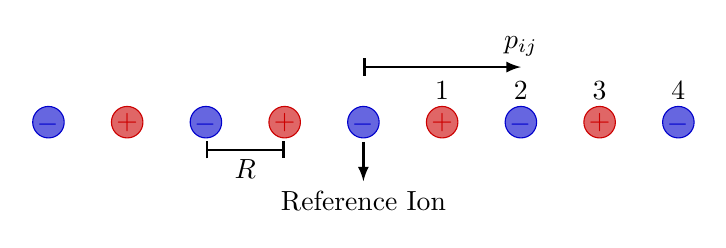
\begin{tikzpicture}
            \foreach \x in {-2, 0, ..., 4} {
                \draw[positive red, fill=positive red!60] (\x, 0) circle [radius=0.2cm];
                \node[positive red] at (\x, 0) {\(+\)};
                \draw[negative blue, fill=negative blue!60] (\x + 1, 0) circle [radius=0.2cm];
                \node[negative blue] at (\x - 0.01 + 1, -0.03) {\(-\)};
            }
            \draw[negative blue, fill=negative blue!60] (-3, 0) circle [radius=0.2cm];
            \node[negative blue] at (-3 - 0.01, 0 - 0.03) {\(-\)};
            \draw[->, thick] (1, -0.25) -- ++ (0, -0.5) node[below] {Reference Ion};
            \draw[|-|, thick] (-1, -0.35) -- (0, -0.35) node[midway, below] {\(R\)};
            \foreach \i in {1, ..., 4} {
                \node at (1 + \i, 0.4) {\i};
            }
            \draw[|->, thick] (1, 0.7) -- ++ (2, 0) node[above] {\(p_{ij}\)};
        \end{tikzpicture}
        \caption{One-dimensional crystal of alternating positive and negative ions.}
        \label{fig:1d ionic crystal}
    \end{figure}
    
    Computing the Madelung constant in higher dimensions is more tricky.
    As a start point summing in order of nearest neighbours doesn't work very well since the terms will oscillate from positive to negative.
    A better method is to sum over spherical shells.
    The resulting sum is conditionally convergent, and when it does converge it doesn't do so particularly quickly since the Coulomb potential goes as \(1/r\) and the number of ions in a spherical shell of radius \(r\) goes as \(r^2\).
    Fortunately we know that \ce{NaCl}, and other structures, exist and therefore we can assume that the sum converges.
    
    A better method for calculating the Madelung constant is the Ewald method.
    It involves transforming the sum to Fourier space for the calculation, and it turns out the convergence is much quicker in Fourier space.
    This method is used by most modern programs for crystal structure calculations.
    
    \subsection{Different Ionic Crystals}
    So far we have considered only \ce{NaCl}, and other crystals of a similar form.
    There are various ionic crystal structures, we typically identify these structures by the most common example.
    The three most common ionic crystal structures are the rock salt type, of which \ce{NaCl} is an example, caesium chloride type, \ce{CsCl}, and zinc blende, \ce{ZnS}.
    
    One scheme for crystal naming is the \define{\textit{Struktubericht} symbols}\index{Struktubericht symbols@\textit{Struktubericht} symbols}.
    In this scheme \(\mathrm{A}\) refers to crystals of a single atom, \(\mathrm{B}\) to crystals of two elements in an equal ratio, \(\mathrm{C}\) to crystals of two elements in a two-to-one ratio, and \(\mathrm{D})\) for all other stoichiometry.
    As well as this there is a number.
    So \(\mathrm{A1}\) is FCC, \(\mathrm{A2}\) is BCC, \(\mathrm{A3}\) is HCP.
    However, we are interested in ionic crystals of equal stoichiometry, so \(\mathrm{B}\).
    Rock salt is of type \(\mathrm{B1}\), \ce{CsCl} is of type \(\mathrm{B2}\), and \ce{ZnS} is of type \(\mathrm{B3}\).
    See \cref{fig:common ionic crystal structures}.
    
    \begin{figure}
        \begin{subfigure}{0.6\textwidth}
            \centering
            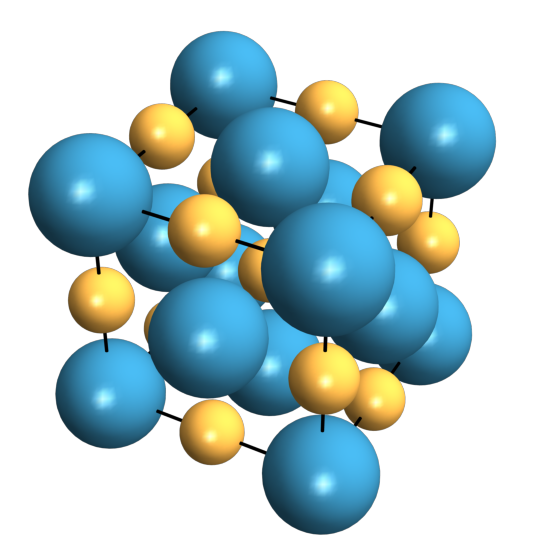
\includegraphics[width=0.6\textwidth]{images/rocksalt.pdf}
            \caption{The rock salt (\(\mathrm{B1}\)) structure.}
        \end{subfigure}
        \begin{subfigure}{0.6\textwidth}
            \centering
            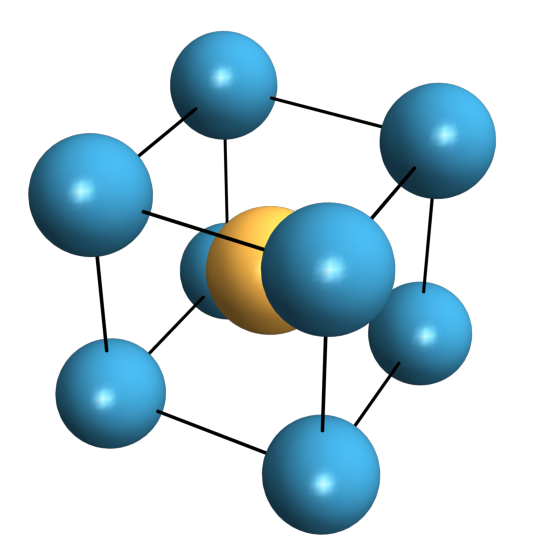
\includegraphics[width=0.6\textwidth]{images/CsCl.pdf}
            \caption{The caesium chloride (\(\mathrm{B2}\)) structure.}
        \end{subfigure}
        \begin{subfigure}{0.6\textwidth}
            \centering
            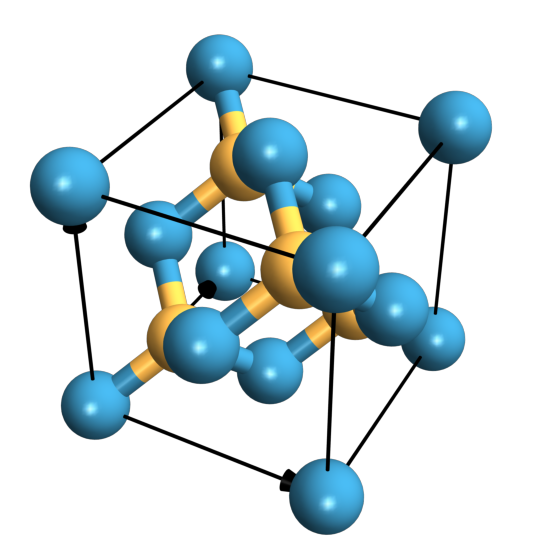
\includegraphics[width=0.6\textwidth]{images/ZnS1.pdf}
            \caption{The zinc blende (\(\mathrm{B3}\)) structure.}
        \end{subfigure}
        \begin{subfigure}{0.6\textwidth}
            \centering
            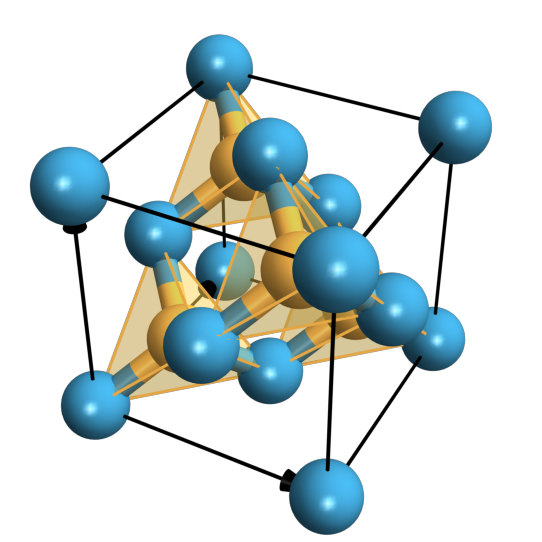
\includegraphics[width=0.6\textwidth]{images/ZnS2.pdf}
            \caption{The zinc blende (\(\mathrm{B3}\)) structure.}
        \end{subfigure}
        \caption{The three most common ionic crystal structures, the rock salt, \ce{CsCl}, and \ce{ZnS} types, also known as \(\mathrm{B1}\), \(\mathrm{B2}\), and \(\mathrm{B3}\).}
        \label{fig:common ionic crystal structures}
    \end{figure}
    
    In all three of these structures both ions have the same local environment.
    That is, each ion is surrounded by the other ion in the same way such that if you swapped the ions the crystal wouldn't change.
    Ions of a similar size tend to form the \ce{CsCl} type whereas ions with a larger size difference tend to form the rock salt type.
    
    The \ce{ZnS} structure is the same as diamond but if you replaced half of the atoms in diamond with a different type.
    This structure is common amongst semiconductors used in optoelectronics (such as LEDs\glossary[acronym]{LED}{light emitting diode}), such as \ce{GaAs}, \ce{GaN}, and \ce{GaP}.
    This type of structure is often found in materials with mixed ionic and covalent bonding.
    
    \subsection{Ionic Spacing}
    We can find the equilibrium spacing between ions by finding the value of \(R\) which minimises \(U_{\tot}\).
    To do so we need to choose a repulsive potential, we choose \(V_{\mathrm{r}}(R) = \lambda\e^{-R/\rho}\).
    We then have
    \begin{equation}
        0 = \diff{U_{\tot}}{R}[R=R_0] = N\left[ -\frac{z\lambda}{\rho}\e^{-R_0/\rho} + \alpha\frac{q^2}{4\pi\varepsilon_0R_0^2} \right].
    \end{equation}
    Rearranging this we have
    \begin{equation}
        \left( \frac{R_0}{\rho} \right)^{2} \e^{-R_0/\rho} = \frac{1}{4\pi\varepsilon_0}\frac{\alpha q^2}{\rho z\lambda}.
    \end{equation}
    This has no analytic solution.
    Numerical solutions give \(R_0/\rho \approx 10\).
    Notice that making either \(\alpha\) or \(q\) larger will make the crystal denser.
    The equilibrium energy is
    \begin{equation}
        U_{\tot}(R_0) = -N\alpha\frac{q^2}{4\pi\varepsilon_0R_0}\left( 1 - \frac{\rho}{R_0} \right).
    \end{equation}
    
    As an example consider \ce{KCl}.
    This has the rock salt structure type with \(z = 6\).
    Experimental properties of \ce{KCl} can be reproduced with \(\rho = \qty{0.30}{\angstrom}\) and \(\lambda = \qty{4}{\kilo\electronvolt}\).
    We then find \(R_0 \approx 10\rho = \qty{3}{\angstrom}\).
    
    \section{Covalent Crystals}
    Covalent bonding arises when the atomic wave functions overlap in such a way as to minimise the energy.
    Crudely we think of this as \enquote{sharing electrons}.
    Unlike other bonding types this forms directional bonds.
    
    Covalent bonding is more complicated to describe and rather than give a full quantum mechanical description we will simply make an analogy to the bonding of the \ce{H_2} molecule\footnote{see notes from principles of quantum mechanics course.}
    When two hydrogen atoms are brought together their initial atomic, \(\mathrm{1s}\), wave functions are no longer eigenstates.
    Instead, a new, lower energy, bonding molecular orbital, \(\mathrm{\upsigma_{1s}}\), is formed, as well as a higher energy, anti-bonding molecular orbital, \(\mathrm{\upsigma_{1s}^*}\).
    See \cref{fig:MO H2}.
    The bonding state has anti-parallel spins and a symmetric wave function, for this reason it is sometimes referred to as an S state.
    The anti-bonding state has parallel spins and an antisymmetric wave function, for this reason it is sometimes referred to as an A state.
    For a covalently bonded molecule to be stable the energy must decrease when the wave functions overlap.
    For this reason \ce{H_2} is stable but \ce{He_2} is not, since the electrons in the anti-bonding state increase the energy by as much as the electrons in the bonding state decrease it.
    
    \begin{figure}
        \tikzexternaldisable
        \begin{modiagram}
            \atom{left} {1s = {0}}
            \atom{right} {1s = {0}}
            \molecule{1sMO = 0.75; pair}
            \node[left] at ($(1sleft) + (-0.1, 0)$) {\(\mathrm{1s}\)};
            \node[right] at ($(1sright) + (0.1, 0)$) {\(\mathrm{1s}\)};
            \node[below] at ($(1sigma) + (0, -0.1)$) {\(\mathrm{\upsigma_{1s}}\)};
            \node[above] at ($(1sigma*) + (0, 0.1)$) {\(\mathrm{\upsigma_{1s}^*}\)};
            \node[above] at ($(1sigma*) + (0, 1)$) {\ce{H_2}};
        \end{modiagram}
        \begin{modiagram}
            \atom{left} {1s = {0}}
            \atom{right} {1s = {0}}
            \molecule{1sMO = 0.75; pair}
            \node at (3, 0.75) {\(\upharpoonleft\mkern-5mu\downharpoonright\)};
            \node[left] at ($(1sleft) + (-0.1, 0)$) {\(\mathrm{1s}\)};
            \node[right] at ($(1sright) + (0.1, 0)$) {\(\mathrm{1s}\)};
            \node[below] at ($(1sigma) + (0, -0.1)$) {\(\mathrm{\upsigma_{1s}}\)};
            \node[above] at ($(1sigma*) + (0, 0.1)$) {\(\mathrm{\upsigma_{1s}^*}\)};
            \node[above] at ($(1sigma*) + (0, 1)$) {\ce{H_2^{2-}}};
        \end{modiagram}
        \tikzexternalenable
        \caption{Molecular orbital diagrams for \ce{H_2} and \ce{He_2}.}
        \label{fig:MO H2}
    \end{figure}

    \section{Metallic Crystals}
    Metallic bonds are basically more extreme forms of covalent bonds in which the overlap of all wave functions (not just neighbours like in covalent bonds) decrease the energy to form a stable state.
    The valence electrons become delocalised.
    The bonds in a metal are non-directional, unlike covalent bonds.
    We will give a fuller picture later where we treat the delocalised electrons like a Fermi gas.
    
    \section{Mixed Binding}
    So far we have only considered one type of bonding at a time.
    In reality all types of bondings occur at once.
    Van der Waaals bonding is weak enough that most of the time it is negligible compared to the other bonding types.
    The refractory metals (a subset of the d-block transition metals including \ce{Mo} and \ce{W}) have high melting points and hardness since they are a mix of metallic and covalently bonded.
    Many metal-non-metal crystals mix covalent and ionic bonding in various amounts, ranging from almost pure covalent bonding for \ce{Si} to about one third ionic bonding for \ce{GaAs}, to two thirds for \ce{ZnS}, to almost pure ionic for \ce{NaCl}.
    
    One interesting case of mixed bonding is graphite.
    In graphite carbon, which is usually \(\mathrm{1s^22s^22p^4}\), forms \(\mathrm{1s^22s^22p^2}\) valence electrons an \(\mathrm{sp^2}\) hybrid orbitals (covalent bonding) and a delocalised electrons (metallic bonding).
    This holds together layers of graphite.
    Between the layers the main bonding effect is van der Waals bonding.
    This leads to graphites interesting properties like being very conductive along the layers but not across and individual layers being strong but still being soft over all as the layers can easily move past each other.
    
    % Appendicies
    \appendixpage
    \begin{appendices}
            \chapter{Constants and Useful Values}

\begin{table}[htb]
    \renewcommand{\arraystretch}{1.2}
    \caption{Important Constants and Their Values. Note masses in electron volts have implicit factors of \(c\).}
    \begin{tabular}{ccl}\toprule
        Constant & Symbol & Value \\\midrule
        Speed of Light & \(c\) &
        \qty{2.99792458e8}{\metre\per\second} \\
        \midrule
        \multirow{2}{*}{Planck Constant} & \multirow{2}{*}{\(h\)} & \qty{6.62607015e-34}{\joule\second} \\
        && \qty{4.135667696}{\electronvolt\second} \\\cline{3-3}
        \multirow{2}{*}{Reduced Planck Constant} & \multirow{2}{*}{\(\hbar\)} & \qty{1.054571817e-34}{\joule\second} \\
        && \qty{6.582119569e-16}{\electronvolt\second}\\
        \midrule
        \multirow{2}{*}{Electron Mass} & \multirow{2}{*}{\(\electronmass\)} & \qty{9.1093837015e-31}{\kilogram} \\
        && \qty{510.99895}{\kilo\electronvolt} \\\cline{3-3}
        \multirow{2}{*}{Elementary Charge} & \multirow{2}{*}{\(e\)} & \qty{1.602176634e-19}{\coulomb} \\
        && \qty{4.80320425e-10}{\statcoulomb} \\
        \midrule
        Electric Constant & \(\varepsilon_0\) & \qty{8.8541878128e-12}{\farad\per\metre} \\
        \midrule
        \multirow{2}{*}{Boltzmann Constant} & \multirow{2}{*}{\(\boltzmann\)} & \qty{1.380649e-23}{\joule\per\kelvin} \\
        && \qty{8.617333262}{\electronvolt\per\kelvin}\\\cline{3-3}
        Molar Gas Constant & \(R\) & \qty{8.314462618}{\joule\per\mole\per\kelvin} \\
        Avogadro Constant & \(\avogadro\) & \qty{6.02214076e23}{\per\mole}\\
        \bottomrule
    \end{tabular}
    \renewcommand{\arraystretch}{1}
\end{table}

\begin{table}[htb]
    \caption{Some unit conversions. Note masses in electron volts have implicit factors of \(c\).}
    \begin{align*}
        \qty{1}{\kilogram} &= \qty{5.609e29}{\mega\electronvolt} & \qty{1}{\mega\electronvolt} &= \qty{1.783e-30}{\kilogram}\\
        \qty{1}{\kilogram} &= \qty{6.022e26}{\dalton} = \qty{6.022e26}{\atomicmassunit} & \qty{1}{\dalton} &= \qty{1}{\atomicmassunit} \qty{1.661e-27}{\kilogram}\\
        \qty{1}{\joule} &= \qty{6.242e18}{\electronvolt} & \qty{1}{\electronvolt} &= \qty{1.602e019}{\joule}\\
        \qty{1}{\metre} &= \qty{e10}{\angstrom} & \qty{1}{\angstrom} &= \qty{e-10}{\metre}
    \end{align*}
\end{table}

\begin{figure}
    \centering
    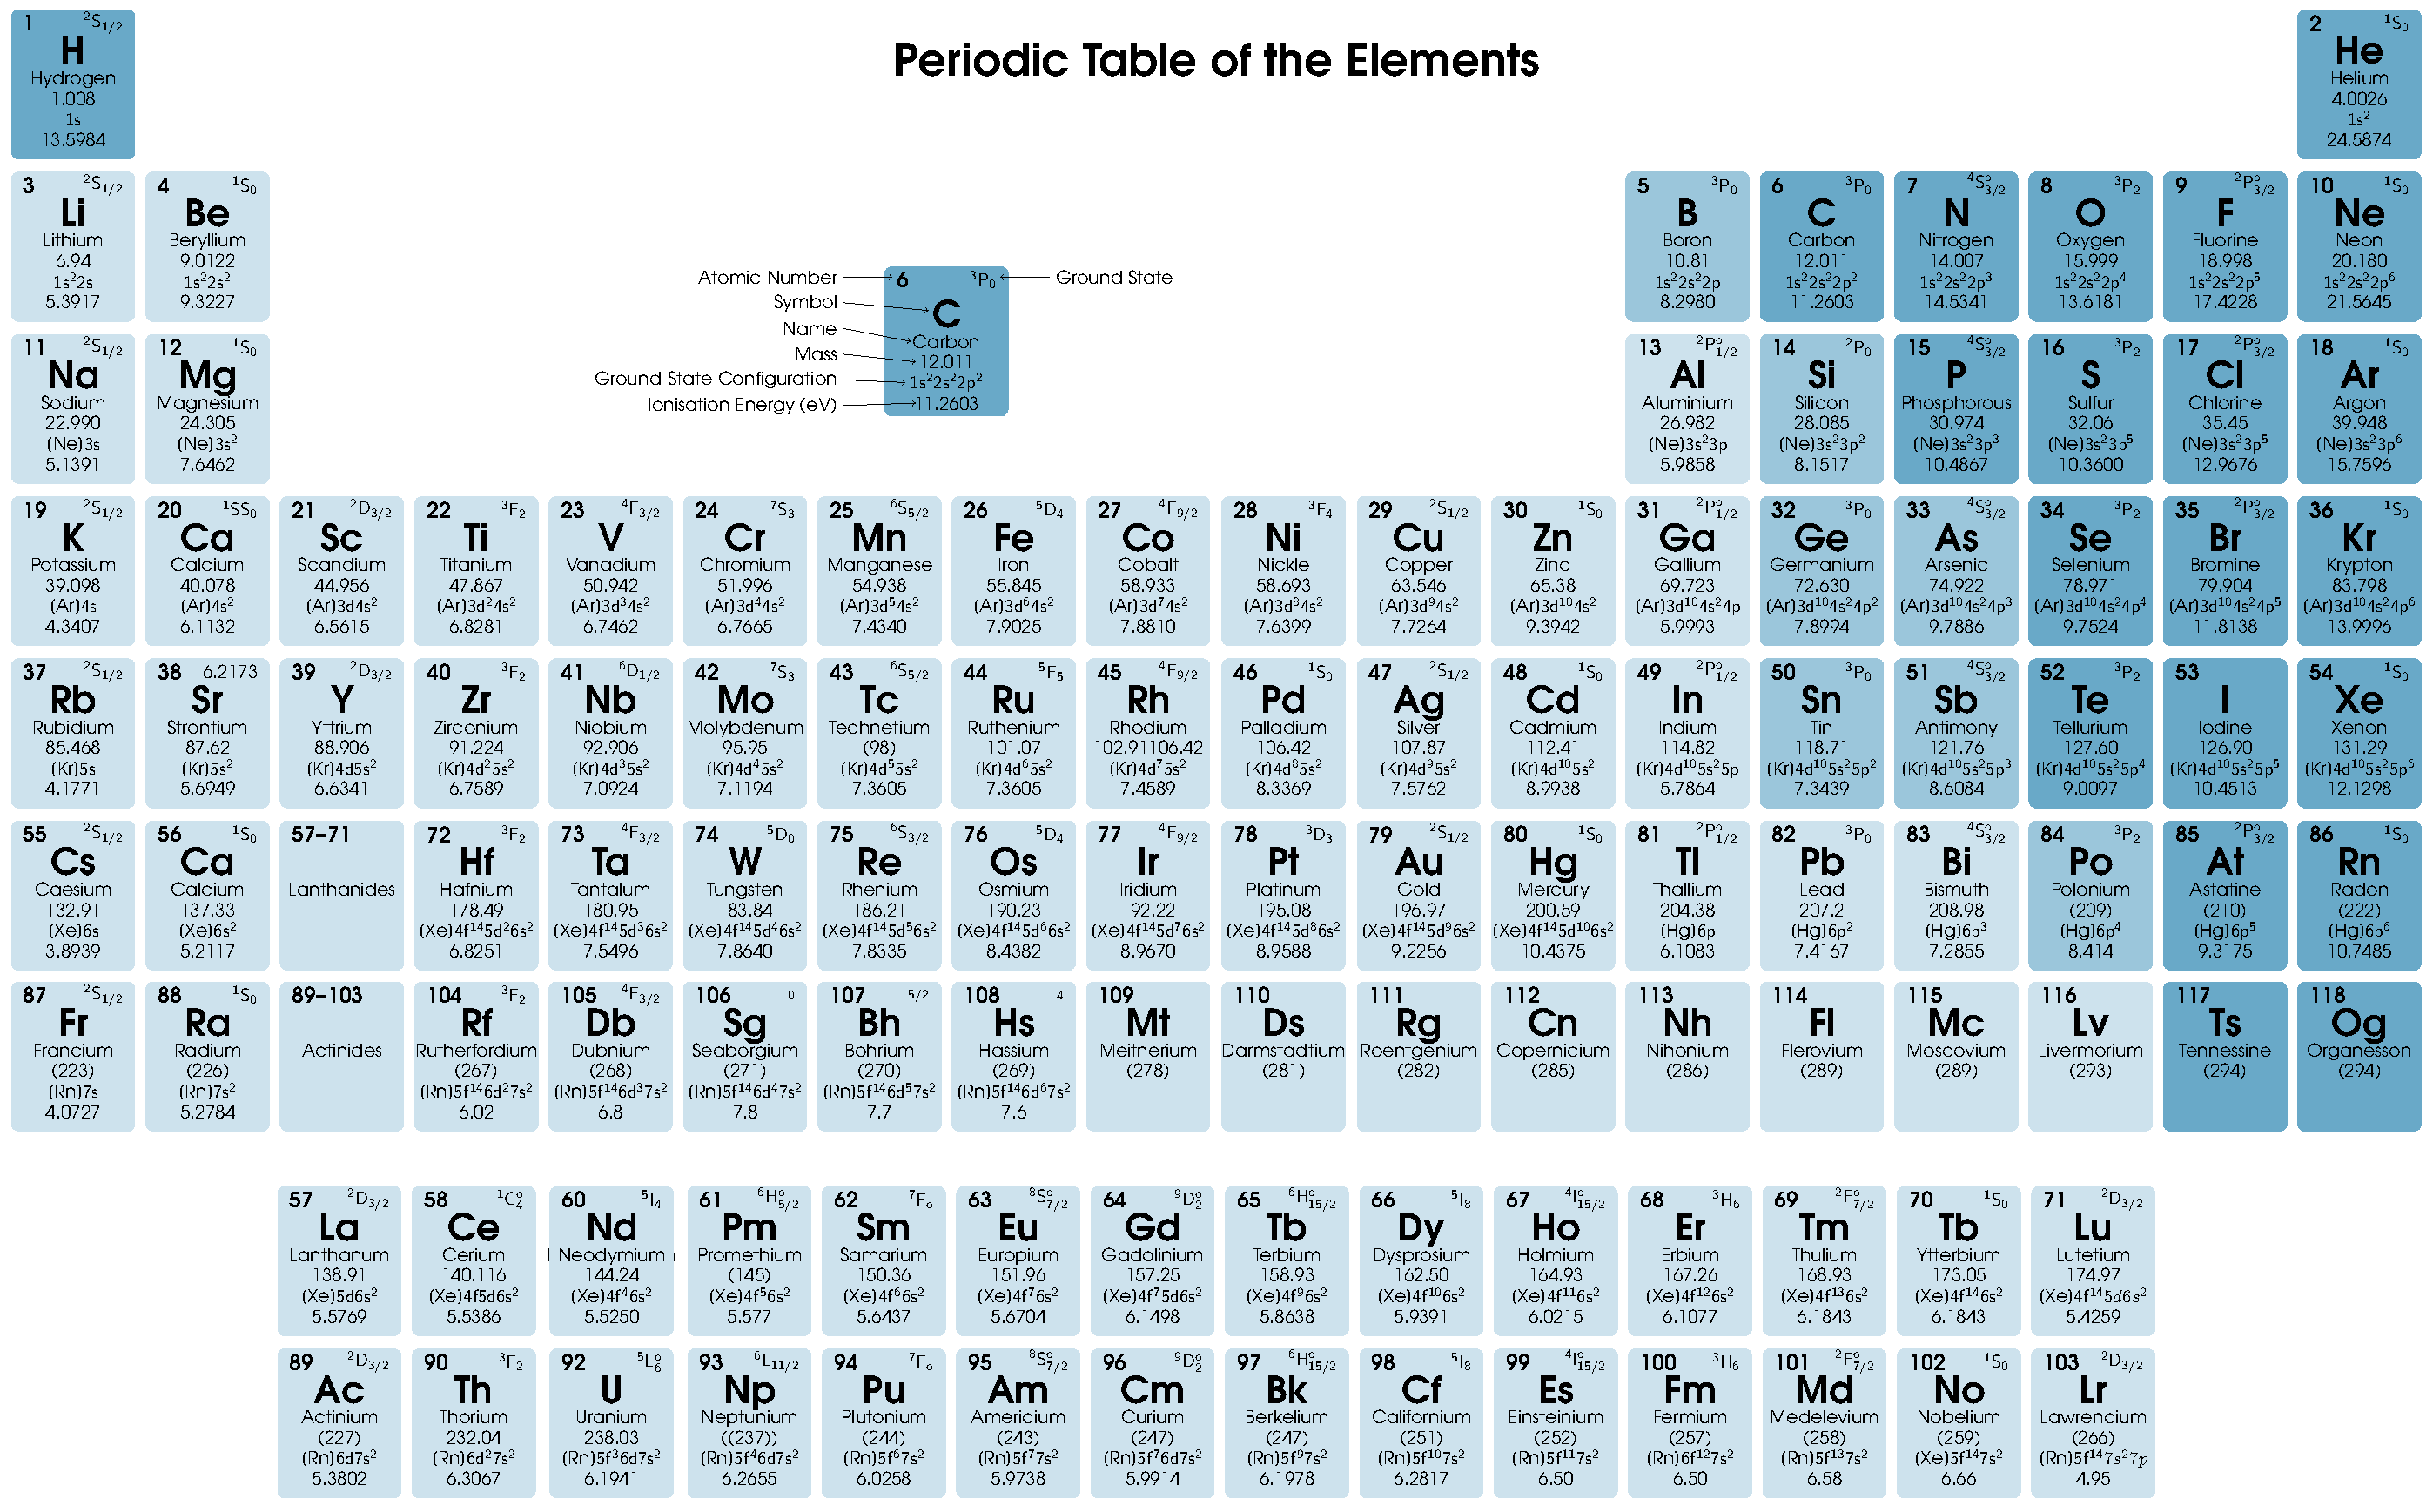
\includegraphics[height=\textwidth, angle=90]{images/periodic-table/periodic-table.pdf}
    \tikzexternaldisable
    \caption{Periodic table of the elements: \protect\tikz{\fill[highlight!20] (0, 0) circle [radius = 0.1];} Metals; \protect\tikz{\fill[highlight!40] (0, 0) circle [radius = 0.1];} Metaloids; \protect\tikz{\fill[highlight!60] (0, 0) circle [radius = 0.1];} Nonmetals.}
    \tikzexternalenable
\end{figure}
        \includ
    \end{appendices}

    \backmatter
    \renewcommand{\glossaryname}{Acronyms}
    \printglossary[acronym]
    \printindex
\end{document}
